% ****** Start of file dressed_quantum_hall.tex ****** %

\documentclass[
 reprint,
 amsmath,amssymb,
 aps,
 prb,
]{revtex4-2}

%===============================================================================
% Import packages
%===============================================================================
% Bold math
\usepackage{bm}
% AMS packages
\usepackage{amsfonts}
\usepackage{amsmath}
\usepackage{amssymb}
\usepackage{mathtools}
% Physics package
\usepackage{physics}
% SI units package
\usepackage{siunitx}
% Hypertext package
\usepackage[breaklinks=true,colorlinks=true,linkcolor=blue,urlcolor=blue,citecolor=blue]{hyperref}
% Language and font encodings
\usepackage[english]{babel}
\usepackage[utf8x]{inputenc}
\usepackage[T1]{fontenc}
%===============================================================================
% Bibliography style
\bibliographystyle{apsrev4-2}

\begin{document}

\preprint{APS/123-QED}

%===============================================================================
% Title of the manuscript
%===============================================================================
\title{A generalized model for the charge transport properties of dressed quantum Hall systems}
%===============================================================================

%===============================================================================
% Authors of the manuscript
%===============================================================================
\author{Kosala Herath,}
\email{kosala.herath@monash.edu}
\author{Malin Premaratne}
\email{malin.premaratne@monash.edu}
\affiliation{Advanced Computing and Simulation Laboratory (A$\chi$L), Department of Electrical and Computer Systems Engineering, Monash University, Clayton, Victoria 3800, Australia.}
%===============================================================================

%===============================================================================
% Add date
%===============================================================================
\date{\today}
%===============================================================================

%===============================================================================
% Abstract
%===============================================================================
\begin{abstract}
We present a generalized mathematical model for predicting the transport properties of a quantum system exposed to a stationary magnetic field and a high-intensity electromagnetic field.
The new formulation, which applies to two-dimensional(2D) dressed quantum Hall systems, is based on Landau quantization theory and Floquet-Drude conductivity approach.
We model our system as a two-dimensional electron gas (2DEG) that interacts with two external fields. To analyze the strong light coupling with the 2DEG, we employ the Floquet theory as a nonperturbative procedure.
Moreover, the Floquet-Fermi golden rule is adopted to explore the impurity scattering effects on charge transport in disordered quantum Hall systems.
We derive fully analytical expressions to describe longitudinal components in the conductivity tensor in dressed quantum Hall systems.
Subsequently, we demonstrate that the conductivity characteristics of quantum Hall systems can be manipulated using strong external light.
Our results align with well-established and experimentally
verified theoretical descriptions for undressed systems while providing a more generalized analysis of the conductivity characteristics in quantum Hall systems.
Thus, our model can be applied to accurately interpret the usage of strong external radiation as a tool in nanoscale quantum devices.
\end{abstract}
%===============================================================================

%===============================================================================
% Make title of the manuscript
%===============================================================================
\maketitle
%===============================================================================

%===============================================================================
% Section 01 : Introduction
%===============================================================================
\section{\label{sec:introduction} Introduction}

Manipulating light-matter interactions in the quantum regime paved the path for an astonishing number of useful technologies in the last century. Quantum optics, which study these interactions, have drawn research attention to the disciplines of optoelectronics \cite{liu16,wijesekara20,tao21,wijesekara21}, sensing \cite{rodrigo15,pirandola18,hapuarachchi2018}, energy harvesting \cite{weeraddana15,yuan16,sun18},
quantum computing \cite{huh15,slussarenko19,andersen21}, bio-information \cite{marais18,bian20}, and many other specialities of recent technologies \cite{rivera20}.
The studies on quantum optics of nanostructures were generally centered on metamaterials \cite{shalaev07,si14}, quantum plasmonic effects \cite{hapuarachchi19,perera20}, lasers and amplifiers \cite{chow13,jayasekara16,premaratne17}, and quantum cavity physics \cite{tsang10,liu17,devi20}.
However, in recent years, one of the foremost aims of examining nanostructures under external radiation was understanding their electron transport characteristics \cite{kitagawa11,zhou11,kibis14,pervishko15,morina15,dehghani15,dini16,wackerl20}.

Better understanding the fundamental mechanisms of charge transport can allow us to invent novel nanoelectronic devices and optimize their performance \cite{premaratne21}.
Most recent studies on the subject have considered the driving field as a perturbation field \cite{pervishko15,morina15}. However, this assumption breaks down for systems under high-intensity illuminations \cite{grifoni98,wackerl20}.
Modeling an electromagnetic field under a perturbative formalism involves expanding the interaction terms in powers of the field intensity. At high intensities, the higher-order terms influence the physics more strongly and the basis of the perturbative treatment begins to break down.
In these instances, a more accurate treatment needs to be adopted. Thus, we treat the interacting fermion system and the radiation as one combined quantum system, namely dressed system \cite{morina15,cohen98,scully01}. Here the applied high-intensity  electromagnetic field identify as the \textit{dressing field}.

Theoretical analyses on the transport properties of dressed fermion systems were recently reported in Refs. \cite{kibis14,morina15,wackerl20}.
Furthermore, in Ref. \cite{wackerl20} a general expression for conductivity in a dressed system has been derived in a fully closed analytical form. In their study, a novel type of Green’s functions, namely four-times Green’s functions were used to derive the Floquet-Drude conductivity formula. This opened the path for exploring and exploiting nanostructures' charge transport attributes under an intense dressing field.

Quantum Hall effect \cite{girvin90} observed in two-dimensional (2D) fermion systems at low temperatures under strong stationary magnetic fields manifest remarkable magneto-transport behaviors. Transport properties of these systems have recently attracted both theoretical \cite{ando72,ando74_1,ando74_2,ando74_3,ando74_4,ando82,endo09} and experimental \cite{allerman95,tieke97,pan05} interest.
Endo \textit{et al.} \cite{endo09} presented the calculations of longitudinal and transverse conductivity tensor components and their relationship in a quantum Hall system. These theoretical calculations  align better with experimental observations compared to previous studies.

In contrast, we can observe more exciting phenomena by simultaneously applying a dressing field to a quantum Hall system already under a non-oscillating magnetic field.
Whilst there exist several leading theories for calculating conductivity tensor elements in quantum Hall systems \cite{ando74_1,ando82,endo09}, these studies  have not been utilized to describe the optical manipulation of charge transport.
Recently, Dini \textit{et al.} \cite{dini16} have investigated the one-directional conductivity behavior of dressed quantum Hall systems. However, they have not adopted the state-of-the-art model to describe the conductivity in a quantum Hall system. In their study, they used the conductivity models from Refs. \cite{ando74_1,ando82}, and as mentioned in Endo \textit{et al.} \cite{endo09}, those models predict a semi-elliptical broadening against Fermi level for each Landau level and provide less agreement with the empirical results.

In the present analysis, we introduce a robust mathematical model for a dressed two-dimensional electron gas (2DEG) subject to another nonoscillating magnetic field.
A stationary magnetic field is applied perpendicularly across the surface of the 2DEG system. This causes the orbital motion of the electrons to be quantized, and a discrete energy spectrum with Landau splitting is observed \cite{landau30}.
In this study, we explicitly calculate the longitudinal components ($\sigma^{xx},\sigma^{yy}$) of the conductivity tensor in a periodically driven quantum Hall system by developing a generalized analytical description using the Floquet-Drude conductivity \cite{wackerl20}.
Finally, we demonstrate that our generalized model reproduces the results of the state-of-the-art conductivity model in Ref. \cite{endo09}, which was developed for the more specific case of quantum Hall systems without the external dressing field.
Moreover, we find that the optical field can be used as a mechanism to regulate transport behavior in numerous 2D nanostructures which can serve as a basis for many useful nanoelectronic devices. We believe that our theoretical analysis and visual depictions of numerical results will lead to a better understanding of manipulating charge transport. Moreover, this will inspire advanced  developments in nanoscale quantum devices.

The paper is organized as follows. Sec.  \ref{sec:schrodinger_problem} introduces our dressed quantum Hall system and the exact wave function solutions for the given configuration. Sec. \ref{sec:floquet_theory} provides the Floquet theory interpretation of these wave functions.
We introduce Floquet-Fermi golden rule for a quantum Hall system in Sec. \ref{sec:inverse_scattering_time}, and use it in Sec. \ref{sec:floquet_drude_conductivity} to derive analytical expressions for longitudinal components of conductivity.
The derived theoretical model is further analyzed numerically using empirical system parameters and compared with previous studies in Sec. \ref{sec:manipulate_conductivity}.
In Sec. \ref{sec:conclusions}, we summarize our analysis and present our conclusions.
%===============================================================================

%===============================================================================
% Section 02 : Schrodinger problem for a dressed quantum Hall system
%===============================================================================
\section{\label{sec:schrodinger_problem} Schrodinger Problem for a Dressed Quantum Hall System}

Our system consists of a 2DEG placed on the $xy$-plane of the three-dimensional coordinate space. In our analysis, the 2DEG is subjected to a nonoscillating magnetic field $\vb{B} = (0,0,B)^{T}$, which is pointed towards the $z$-axis. In addition, a linearly polarized strong light is applied perpendicular to the 2DEG surface. We specially select the frequency of the dressing field $\omega$ to be in the off-resonant regime such that the field behaves as a purely dressing field. Furthermore, without limiting the generality, we choose a $y$-polarized electric field $\vb{E} = (0,E\sin(\omega t),0)^{T}$ for the linearly polarized dressing field as given in Fig.~\ref{fig:1}.
\begin{figure}[b]
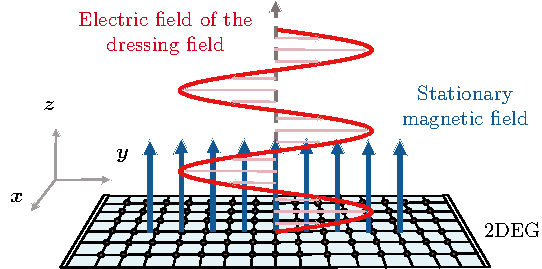
\includegraphics[scale=0.9]{fig_1_system_diagram}
\caption{\label{fig:1} Our 2DEG system only confined in the $xy$-plane while both of the stationary magnetic field $\vb{B}$ and the dressing field are applied perpendicular to the plane of 2DEG. The dressing field is linearly polarized with a $y$-polarized electric field $\vb{E}$.}
\end{figure}
Here $B$ and $E$ represent the amplitudes of the stationary magnetic field and oscillating electric field, respectively.

Using Landau gauge for the stationary magnetic field, we can represent it as a vector potential $\vb{A}_{s} = (-By,0,0)^{T}$. Furthermore, we model the dynamic dressing field in the Coulomb gauge as $\vb{A}_{d}(t) = (0,[E\cos(\omega t)]/\omega,0)^{T}$. These vector potentials are coupled to the momentum of 2DEG as kinetic momentum \cite{mahan00,bruus04}. Thus, we can represent our system with a time-dependent Hamiltonian
\begin{equation} \label{eq:1}
  \hat{H}_e(t) =
  \frac{1}{2m_e}
  \left\{ \hat{\vb{p}} - e\right[ \vb{A}_{s}+\vb{A}_{d}(t) \left] \right\}^2,
\end{equation}
where $m_e$ is the effective electron mass, $e$ is the magnitude of the electron charge, and $\hat{\vb{p}} = (\hat{p}_x,\hat{p}_y,0)^{T}$ represents the canonical momentum operator for 2DEG with electron momentum $(p_{x},p_{y},0)^{T}$.
The exact solutions for the time-dependent Schrödinger equation $i\hbar \dv*{\psi}{t} = \hat{H}_e(t)\psi$ were already derived in Refs. \cite{husimi53,ditt98,dini16}. Here we present them as a set of wave functions defined by two quantum numbers $(n,m)$
\begin{equation} \label{eq:2}
  \begin{aligned}
    &\psi_{n,m}(x,y,t)  \\
      & \quad = \frac{1}{\sqrt{L_x}}
        \chi_n \bm{\left(} y - y_0 - \zeta(t) \bm{\right)}\\
      & \qquad \times
        \exp \bm{\left(}
        \frac{i}{\hbar}\left\{- \epsilon_n t
        + p_x x + \frac{eE}{\omega}(y - y_0)\cos(\omega t) \right.\right.\\
      & \left.\left. \qquad\qquad +
        m_e\dot{\zeta}(t)\left[y - y_0 -\zeta(t)\right] +
        \int_0^{t}L(\zeta,\dot{\zeta},t')\,dt' \right\}\bm{\right)},
  \end{aligned}
\end{equation}
where $n \in \mathbb{Z}^+_0$ and $m \in \mathbb{Z}$. Here $L_{x}$ and $L_{y}$ are dimensions of the 2DEG surface, and $\hbar$ is the reduced Planck constant. The center of the cyclotron orbit on the $y$-axis is given by $y_0 = \flatfrac{-p_x}{(eB)}$ with $p_x = \flatfrac{2\pi\hbar m}{L_x}$.
Moreover, $\chi_n$ are well-known eigenstate solutions for the Schrödinger equation of the stationary quantum harmonic oscillator
\begin{equation} \label{eq:3}
  \chi_n(y) =
  \left( \frac{\kappa}{2^{n}n! \sqrt{\pi}}\right)^{1/2}
  e^{-\kappa^2 y^2/2}
  \mathcal{H}_n \qty(\kappa y),
\end{equation}
with eigenvalues $\epsilon_n = \hbar \omega_0 [n + (1/2)]$ where $\kappa = \sqrt{{m_e \omega_0}/{\hbar}}$, $\mathcal{H}_n(\cdot)$ is the $n$-th Hermite polynomial, and the cyclotron frequency $\omega_0 = eB/m_e$.
We represent the path shift of the driven classical oscillator $\zeta(t)$ by
\begin{equation} \label{eq:4}
  \zeta(t) = \frac{eE}{m_e(\omega_0^2 - \omega^2)}\sin(\omega t),
\end{equation}
and we introduce $\dot{\zeta}(t) = \pdv*{\zeta(t)}{t}$ for the sake of notational ease. We can identify the Lagrangian of the driven classical oscillator $L(\zeta,\dot{\zeta},t)$ as
\begin{equation} \label{eq:5}
  L(\zeta,\dot{\zeta},t) = \frac{1}{2} m_e\dot{\zeta}^2(t) - \frac{1}{2}m_e\omega_0^2 \zeta^2(t) + eE\zeta(t) \sin(\omega t).
\end{equation}
For details of the full derivation, refer to Appendix \ref{appendix_a}.
The exponential phase shifts in Eq.~(\ref{eq:2}) represent the influence of the stationary magnetic field and dressing field on the electron behavior of our system. Therefore, we can renormalize the magneto-transport characteristics of 2DEG by a nonoscillating magnetic field along with a dressing field.
%===============================================================================

%===============================================================================
% Section 03 : Floquet theory perspective
%===============================================================================
\section{\label{sec:floquet_theory} Floquet Theory Perspective}

Symmetry conditions often give useful insights into the behaviors of physical quantum systems.
For instance, the famous Bloch analysis of electrons in quantum systems introduces a mathematical explanation for quantum systems occupying a discrete translational symmetry in the configuration space. Similarly, Floquet theory gives a mathematical formalism that can be used for translational symmetry in time rather than in space \cite{floquet83,grifoni98,holthaus15}.
The Floquet-Drude conductivity theory was employed recently by Wackerl \textit{et al.} \cite{wackerl20} as a method to analyze the transport properties of quantum systems exposed to strong radiation.
In their work, they have presented more accurate results than the former theoretical descriptions for the conductivity of nanoscale systems in the  presence of a dressing field. Therefore, we apply the Floquet-Drude conductivity theory to analyze our 2DEG system which is subjected to both a stationary magnetic field and a dressing field.

First, we need to identify the \textit{quasienergies} and time periodic \textit{Floquet modes} \cite{grifoni98} for the wave functions given in Eq.~(\ref{eq:2}). By factorizing the wave function into a linearly time-dependent part and a periodic time-dependent part, we present the quasienergies with
\begin{equation} \label{eq:6}
  \varepsilon_{n} =
  \hbar \omega_0 \left(n + \flatfrac{1}{2}\right) - \Delta_{\varepsilon},
\end{equation}
which only depends on a single quantum number $n$. Furthermore, we can recognize the Floquet modes as
\begin{equation} \label{eq:7}
  \begin{aligned}
    \phi_{n,m}(x,y,t) =&
    \frac{1}{\sqrt{L_x}} \chi_{n}\bm{\left(}y - y_0 -\zeta(t)\bm{\right)} \\
    & \times
      \exp \bm{\left(}
      \frac{i}{\hbar}\left\{
      p_x x + \frac{eE}{\omega}(y - y_0)\cos(\omega t) \right.\right. \\
    & \left.\left. \qquad\qquad +
      m_e\dot{\zeta}(t)\left[y - y_0 -\zeta(t)\right] +
      \xi \right\}\bm{\right)},
  \end{aligned}
\end{equation}
with
\begin{equation} \label{eq:8}
  \Delta_{\varepsilon} = \frac{e^2E^2}{4m_e(\omega_0^2 - \omega^2)},
\end{equation}
and
\begin{equation} \label{eq:9}
  \xi = \frac{e^2E^2 \left(3\omega^2 - \omega_0^2 \right)}
  {8m_e\omega(\omega_0^2 - \omega^2)^2} \sin(2\omega t).
\end{equation}
For a detailed derivation, refer to Appendix \ref{appendix_b}.
It is important to note that these Floquet modes are time-periodic ($T=2\pi/\omega$) functions. At resonance $\omega = \omega_0$, the energy levels occupy a continuous spectrum and the quasienergy formalism is no longer valid \cite{popov70}. Therefore, in this work we choose a dressing field frequency obeying the condition $\omega \neq \omega_0$.

Performing the Fourier transform over the confined 2D space, we obtain the momentum space ($k_x,k_y$) representation of Floquet modes
\begin{equation} \label{eq:10}
  \begin{aligned}
    \phi_{n,m}\big(k_x,k_y,t\big)  =&
    \sqrt{L_x}
    \widetilde{\chi}_{n} \bm{\left(}k_y - b\cos(\omega t)\bm{\right) }\\
    & \times
    \exp \bm{\left(} i\xi -ik_y  \left[d\sin(\omega t) + y_0 \right] \bm{\right)},
  \end{aligned}
\end{equation}
where
\begin{equation} \label{eq:11}
  \widetilde{\chi}_{n}(k) =
  i^n \left(\frac{1}{ 2^{n} n! \sqrt{\pi} \kappa}\right)^{1/2}
  e^{-\flatfrac{k^2}{(2 \kappa^2)}}
  \mathcal{H}_{n} \left(\flatfrac{k}{\kappa}\right).
\end{equation}
Here we have introduced new parameters
\begin{equation} \label{eq:12}
  b =
  \frac{eE\omega_0^2}{\hbar\omega(\omega_0^2 - \omega^2)},
\end{equation}
and
\begin{equation} \label{eq:13}
  d =
 \frac{eE}{m_e(\omega_0^2 - \omega^2)}.
\end{equation}
Using Floquet theory, we can re-write the wave functions derived in Eq.~(\ref{eq:2}) as the \textit{Floquet states} in momentum space
\begin{equation} \label{eq:14}
  \psi_{n,m}(k_x,k_y,t) =
  \exp(-\flatfrac{i\varepsilon_{n}t}{\hbar}) \phi_{n,m} (k_x,k_y,t).
\end{equation}
%===============================================================================

%===============================================================================
% Section 04 : Inverse scattering time analysis
%===============================================================================
\section{\label{sec:inverse_scattering_time}  Inverse Scattering Time Analysis}

The Floquet-Fermi golden rule was proposed in Ref. \cite{wackerl20} as an approach to analyze the transport properties of dressed quantum systems with impurities.
However, this theory has not been applied for a dressed quantum Hall system in the previous studies. In this analysis, we use Floquet-Fermi golden rule to identify the effects induced by impurities on the magneto-transport properties.
With the help of $t-t'$ formalism \cite{wackerl20,grifoni98,sambe75,peskin93,althorpe97} and applying Floquet states derived in Eq.~(\ref{eq:14}), we can derive an  expression for $(l,l')$-th element of the inverse scattering time matrix for the $N$-th Landau level as
\begin{widetext}
\begin{equation} \label{eq:15}
  \begin{aligned}
    \left(\frac{1}{\tau(\varepsilon,k_x)}\right)^{ll'}_N = &
    \frac{ \pi \hbar\varrho^2}{e^2B^2} \delta(\varepsilon - \varepsilon_N) \\
    & \times
    \int_{-\infty}^{\infty}
    J_l \bm{\left(} \frac{b\hbar}{eB}({k}_x - k_1) \bm{\right)}
    J_{l'} \bm{\left(} \frac{b\hbar}{eB}({k}_x - k_1) \bm{\right)}
    \left|
    \int_{-\infty}^{\infty}
    \chi_N \left( \frac{\hbar}{eB}k_2 \right)
    \chi_N \bm{\left(} \frac{\hbar}{eB}
    \left( k_1 - {k}_x - k_2 \right) \bm{\right)}
    dk_2 \right|^2 d k_1,
  \end{aligned}
\end{equation}
\end{widetext}
where $\varrho = \eta_{imp} L_x \left[\flatfrac{ V_{imp}}{\pi}\right]^{1/2}$, $\varepsilon$ is a given energy value, $J_l(\cdot)$ are Bessel functions of the first kind with $l$-th integer order, and $\varepsilon_N$ is the energy of the $N$-th Landau level.
A more detailed derivation is given in Appendix \ref{appendix_c}.
We modeled the effect caused by impurities in the considered system as a single perturbation potential.
Since random impurities in a disordered metal offer a better approximation for experimental conditions, we assumed that our perturbation potential is formed by a group of randomly distributed impurities.
Thus, we represented the total scattering potential in the 2DEG as a sum of uncorrelated single impurity potentials $\upsilon(\vb{r})$. Here $\eta_{imp}$ is the number of impurities in a unit area, $V_{imp} = \expval{|V_{{k'}_x,k_x}|^2}_{imp}$ with $V_{{k'}_x,k_x} = \mel**{k'_x}{\upsilon(x) }{k_x}$, and $\braket{x}{k_x} = e^{-ik_x x}$.
Moreover, in this analysis, $\expval{\cdot}_{imp}$ represents the average over the impurity disorder.

Next, we analyze the contribution of the inverse scattering time matrix elements on the transport properties of our system.
Since the disorder in the system can not significantly alter the eigenenergy values of the undressed system \cite{wackerl20}, we can neglect the contribution of all off-diagonal elements in the inverse scattering time matrix. Subsequently, we consider only the central diagonal element (${l=l'=0}$) of the inverse scattering time matrix which has the largest contribution to the transport characteristics. Along with this assumption, we introduce a new parameter as the scattering-induced broadening of the $N$-th Landau level \cite{dini16,endo09}
\begin{equation} \label{eq:16}
 \Gamma^{00}_{N}(\varepsilon,k_x) =
 \hbar \left(\frac{1}{\tau(\varepsilon,k_x)}\right)^{00}_N.
\end{equation}
We can evaluate this as
\begin{widetext}
  \begin{equation} \label{eq:17}
   \begin{aligned}
     &\Gamma^{00}_{N} (\varepsilon,k_x) =
     \frac{ \pi \hbar^2 \varrho^2}{e^2B^2}
     \delta(\varepsilon - \varepsilon_{N})
     \int_{-\infty}^{\infty}
     J_0^2 \bm{\left(} \frac{b\hbar}{eB}({k}_x - k_1) \bm{\right)}
     \left|
     \int_{-\infty}^{\infty}
     \chi_N \left( \frac{\hbar}{eB}k_2 \right)
     \chi_N \bm{\left(} \frac{\hbar}{eB}
     \left( k_1 - {k}_x - k_2 \right) \bm{\right)}
     dk_2 \right|^2 d k_1.
   \end{aligned}
  \end{equation}
In addition, for a scattering scenario taking place within the same Landau level, we are able to present the delta distribution of the energy by the  interpretation \cite{dini16}
\begin{equation} \label{eq:18}
 \delta(\varepsilon - \varepsilon_{N}) \approx
 \frac{1}{\pi \Gamma^{00}_N (\varepsilon,k_x)}.
\end{equation}
Subsequently, we write the central element of inverse scattering time matrix in the more compact form
\begin{equation} \label{eq:19}
  \begin{aligned}
    &\Gamma^{00}_{N}(\varepsilon,k_x) =
     \varrho
      \left[
      \int_{-\infty}^{\infty}
      J_0^2 \bm{\left(} \lambda_1 (k_x - k_1) \bm{\right)}
      \left|
      \int_{-\infty}^{\infty}
      \widetilde{\chi}_{N}\left(\lambda_2 k_2 \right)
      \widetilde{\chi}_{N} \bm{\left(} \lambda_2 (k_1 - k_2 - k_x) \bm{\right)}
      dk_2 \right|^2
      dk_1
      \right]^{-\frac{1}{2}},
  \end{aligned}
\end{equation}
where $ \lambda_1 = \flatfrac{\hbar b}{(eB)}$ and  $\lambda_2 = \flatfrac{\hbar \kappa}{(eB)}$.
To analyze the effects of the dressing field on the scattering-induced broadening, we introduce the normalized $N$-th Landau level scattering-induced broadening as
\begin{equation} \label{eq:20}
    \Lambda_N(k_x) =
    \frac{\Gamma^{00}_N (\varepsilon,k_x)}
    {\Gamma^{00}_{N=0}(\varepsilon,k_x)\big|_{E=0}},
\end{equation}
which we can evaluate with
\begin{equation} \label{eq:21}
    \Lambda_N (k_x) =
    \left[
    \frac
    {
      \int_{-\infty}^{\infty}
      J_0^2 \bm{\left(} \lambda_1 (k_x - k_1) \bm{\right)}
      \left|
      \int_{-\infty}^{\infty}
      \widetilde{\chi}_{N}\left(\lambda_2 k_2 \right)
      \widetilde{\chi}_{N} \bm{\left(} \lambda_2 (k_1 - k_2 - k_x) \bm{\right)}
      dk_2 \right|^2
      dk_1
    }
    {
      \int_{-\infty}^{\infty}
      \left|
      \int_{-\infty}^{\infty}
      \widetilde{\chi}_0 \left(\lambda_2 k_2 \right)
      \widetilde{\chi}_0 \bm{\left(} \lambda_2 (k_1 - k_2 - k_x) \bm{\right)}
      dk_2 \right|^2
      dk_1
    }
    \right]^{1/2}.
\end{equation}
\end{widetext}

\begin{figure}[t]
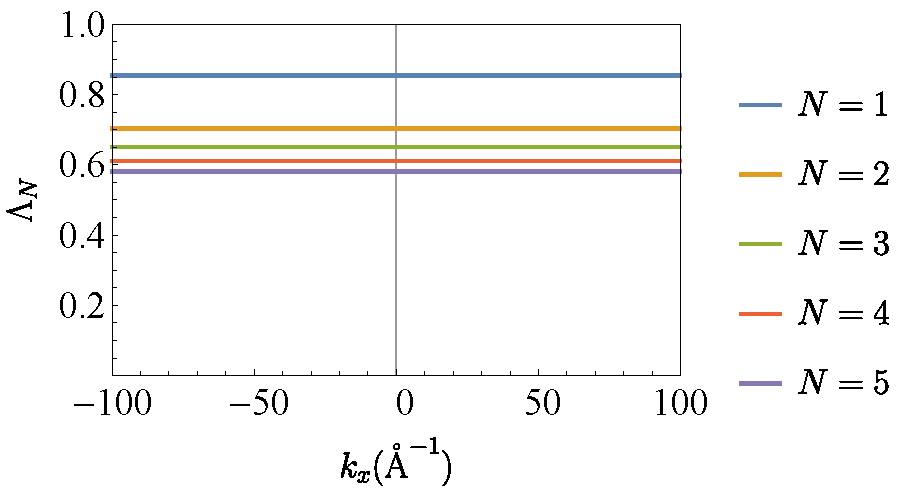
\includegraphics[scale=0.55]{fig_2_normalized_broadening_with_momentum}
\caption{\label{fig_3} The dependence of normalized scattering-induced broadening $\Lambda_N$ for each Landau level ($N =0,1,2,3,4$) against $x$-directional momentum value $k_x$ in a GaAs-based quantum well under a nonoscillating magnetic field with $B = \SI{1.2}{\tesla}$, dressing field with a  frequency of $\omega =\SI{2e12}{\radian\per\second}$ and intensity $I =\SI{100}{\watt\per\square\centi\metre}$.
In this calculation, we have assumed that the natural  broadening of $0$-th Landau level $\Gamma_0$ is $\SI{0.24}{\milli\eV}$.}
\end{figure}

\begin{figure}[t]
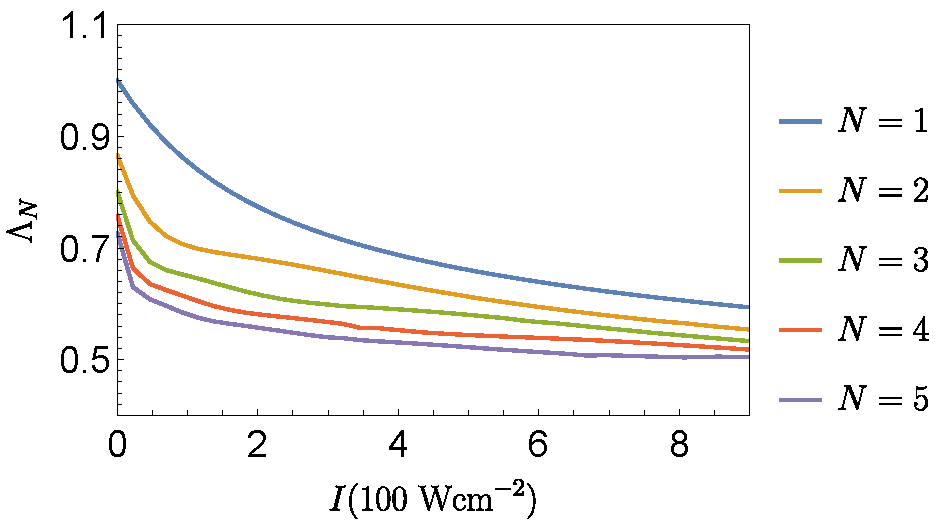
\includegraphics[scale=0.54]{fig_3_normalized_broadening_with_intensity}
\caption{\label{fig_4} The dependence of normalized scattering-induced broadening $\Lambda_N$ for each Landau level ($N =0,1,2,3,4$) against dressing field intensity $I$, in a GaAs-based quantum well under a nonoscillating magnetic field with $B = \SI{1.2}{\tesla}$, dressing field with a frequency of $\omega =\SI{2e12}{\radian\per\second}$. In this calculation, we have assumed that the natural broadening of $0$-th Landau level $\Gamma_0$ is $\SI{0.24}{\milli\eV}$.}
\end{figure}

Next, we calculated the normalized energy band broadening against $x$-directional momentum component ${k_x}$ for different Landau levels ($N = 0,1,2,3,4$) for GaAs-based quantum well and the results are depicted in Fig.~\ref{fig_3} and Fig.~\ref{fig_4}. To make a comparison, we have selected the experiment parameters to match with analysis in Ref.~\cite{endo09}.
In that study, the authors have assumed that the effective mass of the electron in GaAs-based quantum well system is $m_e \approx 0.07\widetilde{m}_e$ where $\widetilde{m}_e$ is the mass of the electron \cite{endo09,winkler03,wackerl20}. In addition, they used the broadening of the undressed $0$-th Landau level $\Gamma_0$ as $\SI{0.24}{\milli\eV}$. Therefore, in our calculations, we assumed that the natural least Landau level broadening also has this value: $\Gamma^{00}_{N=0}|_{E=0} = \SI{0.24}{\milli\eV}$.
Here, we observe that the normalized energy broadening value for each Landau level is independent of the $x$-directional momentum $k_x$ value and we are able to manipulate it by the dressing field. When the dressing field's intensity increases, the energy broadening is reduced, which leads to changes in the transport properties of the dressed quantum Hall system.
To analyze these adjustments in detail, we derive an analytical expression for the conductivity of a dressed quantum Hall system in the next section.
%===============================================================================

%===============================================================================
% Section 05 : Floquet-Drude Conductivity in a Dressed Quantum Hall System
%===============================================================================
\section{\label{sec:floquet_drude_conductivity} Floquet-Drude Conductivity in a Dressed Quantum Hall System}

A general theory for the conductivity of a dressed system with disorder was reported by Wackerl \textit{et al.} \cite{wackerl20,wackerlthesis20}. This theory, the general $x$-directional longitudinal DC-limit conductivity has been characterized as
\begin{equation} \label{eq:22}
  \begin{aligned}
    \sigma^{xx} = &
    \frac{-1}{4\pi\hbar A}
    \int_{\Pi-\hbar\omega/2}^{\Pi+ \hbar\omega/2}
    \left(
    -\pdv*{f}{\varepsilon }\right) \\
    &  \quad\times
    \tr
    \left\{
    {j}^x_0
    \left[
    \vb{G}^{r} (\varepsilon) - \vb{G}^{a} (\varepsilon)
    \right]
    {j}^x_0
    \left[
    \vb{G}^{r} (\varepsilon) - \vb{G}^{a} (\varepsilon)
    \right]
    \right\} d\varepsilon,
  \end{aligned}
\end{equation}
where $j^x_0$ is the $x$-directional electric current operator matrix elements' $0$-th Fourier component. Here, $\vb{G}^{r}(\varepsilon)$ and $\vb{G}^{a} (\varepsilon)$ are the retarded and advanced white noise disorder averaged Floquet Green function matrices \cite{wackerl20,wackerlthesis20}, respectively. These matrices are defined against the Floquet modes of the considering system. Here we have assumed that only $0$-th Fourier component of the current operator is contributing to the conductivity. In addition, $A$ is the area of the considered two-dimensional system, $f$ is the partial distribution function, and $\Pi$ is a function that can be chosen such that
\begin{equation} \label{eq:23}
    \Pi- \flatfrac{\hbar \omega}{2}
    \leq \varepsilon_N
    <
    \Pi + \flatfrac{\hbar \omega}{2}.
\end{equation}
Here $ \varepsilon_N$ are quasienergies of all relevant Floquet states, and $tr\{\cdot\}$ is the trace of the considering operator.

Next, we restrict our analysis into the off-resonant regime $\omega\tau_0 \gg 1$), where $\tau_0$ is the scattering time of the undriven system. Thus, we can expand the $x$-directional longitudinal conductivity given in
Eq.~(\ref{eq:22}) using only the central entry Fourier components ($l=l'=0$) of Floquet modes $\ket{\phi_{n,m}} = \ket{n,k_x}$ as
\begin{widetext}
\begin{equation} \label{eq:24}
  \begin{aligned}
    \sigma^{xx} =
    \frac{-1}{4\pi\hbar A}
    \int_{\Pi-\hbar\omega/2}^{\Pi+ \hbar\omega/2}
    \left(
      -\frac{\partial f}{\partial \varepsilon}
    \right)
    \frac{1}{V_{k_x}} \sum_{k_x}
    \sum_{n}
    \mel{n,k_x}
    {
      {j}^x_0
      \left[
        \vb{G}^{r} (\varepsilon) - \vb{G}^{a} (\varepsilon)
      \right]
      {j}^x_0
      \left[
        \vb{G}^{r} (\varepsilon) - \vb{G}^{a} (\varepsilon)
      \right]
    }
    {n,k_x}
    d\varepsilon,
  \end{aligned}
\end{equation}
where $V_{k_x}$ is the volume of considering $x$-directional momentum space. Next, we evaluate the above expression as follows
\begin{equation} \label{eq:25}
  \begin{aligned}
    \sigma^{xx}  = &
    \frac{-1}{4\pi\hbar A}
    \int_{\Pi-\hbar\omega/2}^{\Pi+ \hbar\omega/2}
    \left(
      -\frac{\partial f}{\partial \varepsilon}
    \right)
    \frac{1}{V_{k_x}^4}
    \sum_{k_x} \sum_{n}
    \sum_{{k_x}_1,{k_x}_2,{k_x}_3}
    \sum_{n_1,n_2,n_3} \\
    & \quad\times \mel{n,k_x}{
    {j}^x_0}
    {n_1,{k_x}_1}
    \mel{{n_1,{k_x}_1}}{
    \left[
      \vb{G}^{r} (\varepsilon) - \vb{G}^{a} (\varepsilon)
    \right]
    }
    {n_2,{k_x}_2}
    \mel{n_2,{k_x}_2}{
    {j}^x_0}
    {n_3,{k_x}_3}
    \mel{n_3,{k_x}_3}{
    \left[
      \vb{G}^{r} (\varepsilon) - \vb{G}^{a} (\varepsilon)
    \right]
    }
    {n,k_x} d\varepsilon.
  \end{aligned}
\end{equation}
We can diagonalize the impurity averaged Green's functions using a unitary transformation ($\vb{T}  = \ket{n,k_x}$) as mentioned in Refs.~\cite{wackerl20,wackerlthesis20,tsuji08}. Thus, we evaluate the matrix elements of the difference between retarded and advanced Green's functions as
\begin{equation} \label{eq:26}
  \mel{{n_1,{k_x}_1}}
  {
    \vb{T}^{\dagger}
    \left[
    \vb{G}^{r} (\varepsilon) - \vb{G}^{a} (\varepsilon)
    \right]\vb{T}
  }
  {n_2,{k_x}_2} =
  \frac
  {
    2i \Im(\vb{T}^{\dagger} \vb{\Sigma}^r \vb{T})
    \delta_{n_1,n_2}\delta_{{k_x}_1,{k_x}_2}
  }
  {
    \left(
    \flatfrac{\varepsilon}{\hbar} -
    \flatfrac{\varepsilon_{n_1}}{\hbar}
    \right)^2
    + \left[\Im(\vb{T}^{\dagger} \vb{\Sigma}^r \vb{T})\right]^2
  },
\end{equation}
and
\begin{equation} \label{eq:27}
  \mel{{n_3,{k_x}_3}}{
  \vb{T}^{\dagger}
  \left[
  \vb{G}^{r} (\varepsilon) - \vb{G}^{a} (\varepsilon)
  \right]\vb{T}}
  {n,{k_x}} =
  \frac{
    2i \Im(\vb{T}^{\dagger} \vb{\Sigma}^r \vb{T})
    \delta_{n_3,n}\delta_{{k_x}_3,{k_x}}
  }
  {
    \left(
    \flatfrac{\varepsilon }{\hbar}-
    \flatfrac{\varepsilon_{n}}{\hbar}
    \right)^2
    + \left[\Im(\vb{T}^{\dagger} \vb{\Sigma}^r \vb{T})\right]^2
  }.
\end{equation}
Here we introduced the retarded self-energy matrix $\vb{\Sigma}^r$ which is the sum of all irreducible diagrams \cite{wackerl20,wackerlthesis20}. Applying the matrix elements of the electric current operator in Landau levels and
expressions from Eq.~(\ref{eq:26}) and Eq.~(\ref{eq:27}) back into Eq.~(\ref{eq:25}) we obtain
\begin{equation} \label{eq:28}
  \begin{aligned}
    \sigma^{xx}  =
    \frac{-1}{4\pi\hbar A}
    \int_{\Pi-\hbar\omega/2}^{\Pi+ \hbar\omega/2}&
    \left(
    -\frac{\partial f}{\partial \varepsilon}
    \right)
    \frac{1}{V_{k_x}}
    \sum_{k_x} \sum_{n} \sum_{n_1,n_2}
    \\
    & \times
    \frac{e^2B}{{m_e}}
    \left(
    \sqrt{\frac{n+1}{2}} \delta_{n_1,n+1} + \sqrt{\frac{n}{2}}\delta_{n_1,n-1}
    \right)
    \left\{
    \frac
    {
      2i \Im(\vb{T}^{\dagger} \vb{\Sigma}^r \vb{T})
      \delta_{n_1,n_2}
    }
    {
      \left(
      \flatfrac{\varepsilon}{\hbar} -
      \flatfrac{\varepsilon_{n_1}}{\hbar}
      \right)^2
      + \left[\Im(\vb{T}^{\dagger} \vb{\Sigma}^r \vb{T})\right]^2
    }
    \right\} \\
    & \times
    \frac{e^2B}{{m_e}}
    \left(
    \sqrt{\frac{n_2+1}{2}} \delta_{n,n_2+1} + \sqrt{\frac{n_2}{2}}
    \delta_{n,n_2-1}
    \right)
    \left\{
    \frac{
      2i \Im(\vb{T}^{\dagger} \vb{\Sigma}^r \vb{T})
    }
    {
      \left(
      \flatfrac{\varepsilon }{\hbar}-
      \flatfrac{\varepsilon_{n}}{\hbar}
      \right)^2
      + \left[\Im(\vb{T}^{\dagger} \vb{\Sigma}^r \vb{T})\right]^2
    }
    \right\}  d\varepsilon,
  \end{aligned}
\end{equation}
For the full derivation of electric current operators in a quantum Hall system, refer to Appendix \ref{appendix_d}.
After the expansion, we can identify the the only non-zero term as follows
\begin{equation} \label{eq:29}
  \begin{aligned}
    \sigma^{xx} =
    \frac{-1}{4\pi\hbar A}
    \frac{e^4B^2}{{{m_e}^2}} &
    \int_{\Pi-\hbar\omega/2}^{\Pi+ \hbar\omega/2}
    \left(
    -\frac{\partial f}{\partial \varepsilon}\right)
    \frac{1}{V_{k_x}} \sum_{k_x} \sum_{n}
    (n+1)
    \\
    & \times
    \left\{
    \frac
    {
      2i \Im\bm{(}\vb{T}^{\dagger} \vb{\Sigma}^r(\varepsilon_{n+1},k_x) \vb{T}\bm{)}
    }
    {
      \left(
      \flatfrac{\varepsilon}{\hbar} -
      \flatfrac{\varepsilon_{n+1}}{\hbar}
      \right)^2
      + \left[\Im\bm{(}\vb{T}^{\dagger} \vb{\Sigma}^r(\varepsilon_{n+1},k_x) \vb{T}\bm{)}\right]^2
    }
    \right\}
    \left\{
    \frac{
      2i \Im\bm{(}\vb{T}^{\dagger} \vb{\Sigma}^r(\varepsilon_n,k_x) \vb{T}\bm{)}
    }
    {
      \left(
      \flatfrac{\varepsilon }{\hbar}-
      \flatfrac{\varepsilon_{n}}{\hbar}
      \right)^2
      + \left[\Im\bm{(}\vb{T}^{\dagger} \vb{\Sigma}^r(\varepsilon_n,k_x) \vb{T}\bm{)}\right]^2
    }
    \right\}
    d\varepsilon.
  \end{aligned}
\end{equation}
The inverse scattering time matrix is equal to the diagonalized contrast of the retarded and advanced self-energy \cite{wackerl20,wackerlthesis20}. In addition, on the diagonal the contrast of the retarded and advanced Green's function can be represented with the imaginary component of the retarded self-energy \cite{wackerl20,wackerlthesis20}. Subsequently, we can identify the following property
\begin{equation} \label{eq:30}
  \left(\frac{1}{\tau(\varepsilon,k_x)}\right)^{ll} =
  -2\text{Im} \left[ \vb{T}^{\dagger} \vb{\Sigma}^r(\varepsilon,k_x) \vb{T}\right]^{ll}.
\end{equation}
Afterwards, considering only the central element ($l=0$) of the inverse scattering time matrix, we can restructure the derived conductivity expression in Eq.~(\ref{eq:29}) as follows
\begin{equation} \label{eq:31}
    \sigma^{xx}   =
    \frac{1}{\pi\hbar A}
    \frac{e^4B^2}{{{m_e}^2}}
    \int_{\Pi-\hbar\omega/2}^{\Pi+ \hbar\omega/2}
    \left(
      -\frac{\partial f}{\partial \varepsilon}
    \right)
    \frac{1}{V_{k_x}} \sum_{k_x} \sum_{n} (n+1)
    \left[
    \frac{\widetilde{{\Gamma}}(\varepsilon_{n+1})
    }
    {
    \left(
    \varepsilon_F - \varepsilon_{n+1}
    \right)^2
    + \widetilde{{\Gamma}}^2(\varepsilon_{n+1})
    }
    \right]
    \left[
    \frac{\widetilde{{\Gamma}}(\varepsilon_{n})
    }
    {
    \left(
    \varepsilon_F - \varepsilon_{n}
    \right)^2
    + \widetilde{{\Gamma}}^2(\varepsilon_{n})
    }
    \right]
    d\varepsilon,
\end{equation}
\end{widetext}
with $\widetilde{{\Gamma}}(\varepsilon_n,k_x) = \left[\flatfrac{\hbar}{2\tau(\varepsilon_n,k_x)}\right]^{00}$. Since we already identified that the inverse scattering time matrix's central element is independent of $k_x$ value, we can drop the $k_x$-dependent in the $\widetilde{{\Gamma}}(\varepsilon_n,k_x)$ terms. Subsequently, we can get the sum over available momentum in $x$-direction.
However, by considering the condition that the center of the cyclotron orbit $y_0$ must physically lie within the considered system, we can identify that
\begin{equation} \label{eq:32}
 -\flatfrac{m_e\omega_0 Ly}{(2\hbar)} \leq k_x \leq \flatfrac{m_e\omega_0 Ly}{(2\hbar)}.
\end{equation}
We use the Fermi-Dirac distribution as our partial distribution function ($f$) for our system
\begin{equation} \label{eq:33}
  f(\varepsilon) = \frac{1}{\exp[(\varepsilon - \varepsilon_F)/k_B T]+1},
\end{equation}
where $k_B$ is the Boltzmann constant, $T$ is the absolute temperature and $\varepsilon_F$ is the Fermi energy of the system. Considering the above distribution for extremely low-temperature conditions, we can use the following approximation
\begin{equation} \label{eq:34}
  - \pdv{f(\varepsilon)}{\varepsilon} \approx \delta(\varepsilon - \varepsilon_F).
\end{equation}
Moreover, let $\Pi = \varepsilon_F$ and the derived expression in Eq.~(\ref{eq:31}) leads to
\begin{equation} \label{eq:35}
  \begin{aligned}
    \sigma^{xx}  =
    \frac{e^2}{\pi\hbar A}
    \sum_{n} &
    \frac{(n+1)}{\gamma_{n}\gamma_{n+1}} \\
    &\times
    \left[
      \frac{1}
      {
        1 + \left(\frac{X_F - n -1}{\gamma_{n+1}}\right)^2
      }
    \right]
    \left[
      \frac{1}
      {
        1 + \left(\frac{X_F - n}{\gamma_{n}}\right)^2
      }
    \right],
  \end{aligned}
\end{equation}
where $X_F = \left[\flatfrac{\varepsilon_F}{(\hbar \omega_0)} - \flatfrac{1}{2}\right]$
and
$\gamma_n = \flatfrac{\widetilde{{\Gamma}}(\varepsilon_n)}{(\hbar \omega_0)}$.
Following the same steps as above derivation, we can derive the longitudinal conductivity in the $y$-direction by applying the electric current operator for $y$-direction derived in Appendix \ref{appendix_d}
\begin{equation} \label{eq:36}
  \begin{aligned}
    {\sigma}^{yy} =
    \frac{e^2}{\pi\hbar A} &
    \frac{1}{e^2B^2}
    \sum_{n}
    \frac{(n+1)}{\gamma_{n}\gamma_{n+1}} \\
    & \times
    \left[
      \frac{1}
      {
        1 + \left(\frac{X_F - n -1}{\gamma_{n+1}}\right)^2
      }
    \right]
    \left[
      \frac{1}
      {
        1 + \left(\frac{X_F - n}{\gamma_{n}}\right)^2
      }
    \right].
  \end{aligned}
\end{equation}
%===============================================================================

%===============================================================================
% Section 06 : Manipulate Conductivity in Quantum Hall Systems
%===============================================================================
\section{\label{sec:manipulate_conductivity} Manipulate Conductivity in Quantum Hall Systems}

To identify the longitudinal conductivity characteristics of quantum Hall system under external dressing field, first we derive an expression for normalized longitudinal conductivity as a function of Fermi energy $X_F$ and intensity of the dressing field $I$.
We can identify the normalized $x$-directional longitudinal conductivity of dressed quantum Hall system by
\begin{equation}\label{eq:37}
  \widetilde{\sigma}^{xx}(X_F,I) =
  \flatfrac{\sigma^{xx}}{\sigma_{0}},
\end{equation}
with $\sigma^0 = \flatfrac{e^2}{(\pi \hbar A)}$, and we can express this as
\begin{equation} \label{eq:38}
  \begin{aligned}
    \widetilde{\sigma}^{xx}(X_F,I) &=
    \sum_{n}
    \frac{(n+1)}{\varsigma^2 \Lambda_n \Lambda_{n+1}} \\
    &\quad\times
    \left[
      \frac{1}
      {
        1 + \left(\frac{X_F - n -1}{\varsigma \Lambda_n}\right)^2
      }
    \right]
    \left[
      \frac{1}
      {
        1 + \left(\frac{X_F - n}{\varsigma \Lambda_{n+1}}\right)^2
      }
    \right],
  \end{aligned}
\end{equation}
where $\varsigma = \flatfrac{\Gamma_0}{(2\hbar \omega_0)}$. Here, $\Gamma_0$ is the natural energy broadening of the least Landau level.

As illustrated in Fig.~\ref{fig:5} and Fig.~\ref{fig:6}, we can manipulate the normalized longitudinal conductivity $\widetilde{\sigma}^{xx}$ with the applied dressing field's intensity and the Fermi level $X_F$ of the considered system.
For a given dressing field intensity, the longitudinal conductivity varies with  the Fermi level of the system showing sharp peaks at each Landau energy level.
In quantum Hall systems, electrons are restricted to bear only the Landau energies. Thus, the conductivity reduces significantly when the Fermi level is not aligned with any of the Landau levels. In contrast, near each Landau level, the conductivity achieves excessive values compared to other areas. Moreover, as illustrates in Fig.~\ref{fig:5}, the peak value of the normalized longitudinal conductivity on each Landau level gets increased with the Landau level number.

On the other hand, considering the effects of the applied dressing field on the longitudinal conductivity of 2DEG, we can identify that the dressing field has sharpened the conductivity peaks.
When we increase the intensity level of the dressing field, the conductivity regions get weakened as illustrated in the Fig.~\ref{fig:6}.
However, the peak value of the conductivity at each Landau level has the same value as the undressed system. This demonstrates our ability to tune the width of the conductivity regions in these quantum Hall systems with the help of a dressing field.

These characteristics align well with the outcomes demonstrated by Dini \textit{et al.} \cite{dini16}.  As the authors remarked in that publication, since the Fermi level of the system can be changed with the applied gate voltage of the material, this can be utilized as a 2D switch for nanoscale optoelectronics applications. Controlling  the external dressing field's intensity allows us to fine-tune this switching mechanism for optimized performance.
However, we can distinguish that the shapes and behavior of the conductivity regions that illustrated in Fig.~\ref{fig:5} and Fig.~\ref{fig:6} are generally incompatible with the results reported in Ref.~\cite{dini16}. This is due to the selection of the conventional longitudinal conductivity theory of 2DEG from Refs.~\cite{ando74_1,ando82}. The semi-elliptical conductivity regions are  illustrated in Refs.~\cite{dini16,ando74_1,ando82}, have less consistency with the experimentally observed data for Landau levels \cite{endo09}.
In our study of the transport properties of quantum Hall systems, we developed the conductivity expression starting from the Floquet-Drude conductivity \cite{wackerl20} and we achieved outcomes that align with the results depicted in Ref. \cite{endo09}.
The theory on the conductivity of quantum Hall systems in Ref.~\cite{endo09} provides an excellent agreement with the experimentally observed results in GaAs/AlGaAs 2DEG for the low magnetic field range.
However, they have not considered the tunability that can be achieved with a dressing field. In this analysis, we account for both the magnetic and dressing field effects that can affect the transport properties of 2DEG, leading to a more generalized theory. Thus in this study, we were able to demonstrate that using Floquet-Drude conductivity method, one can derive a more generalized mathematical model which fits better with experiment for the charge transport properties of quantum Hall systems.

\begin{figure}[t]
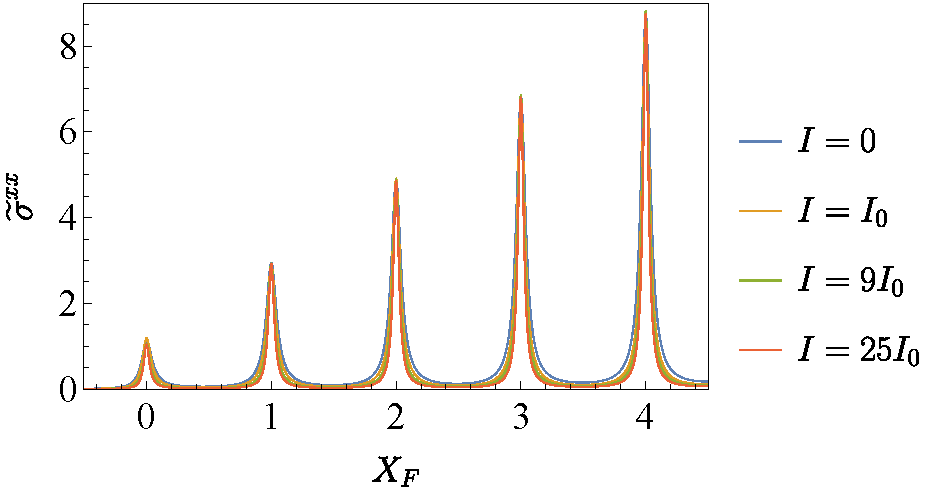
\includegraphics[scale=0.54]{fig_4_conductivity_with_fermi_level}
\caption{ Normalized longitudinal conductivity $\widetilde{\sigma}^{xx}$ against Fermi level $X_F$ with different intensities $I$ of the external dressing field in a GaAs-based quantum well under a nonoscillating magnetic field with $B = \SI{1.2}{\tesla}$, dressing field with a  frequency of $\omega =\SI{2e12}{\radian\per\second}$ and $I_0 =\SI{100}{\watt\per\square\centi\metre}$. In this calculation, we have assumed that the natural  broadening of $0$-th Landau level $\Gamma_0$ is $\SI{0.24}{\milli\eV}$.}
\label{fig:5}
\end{figure}

\begin{figure}[t]
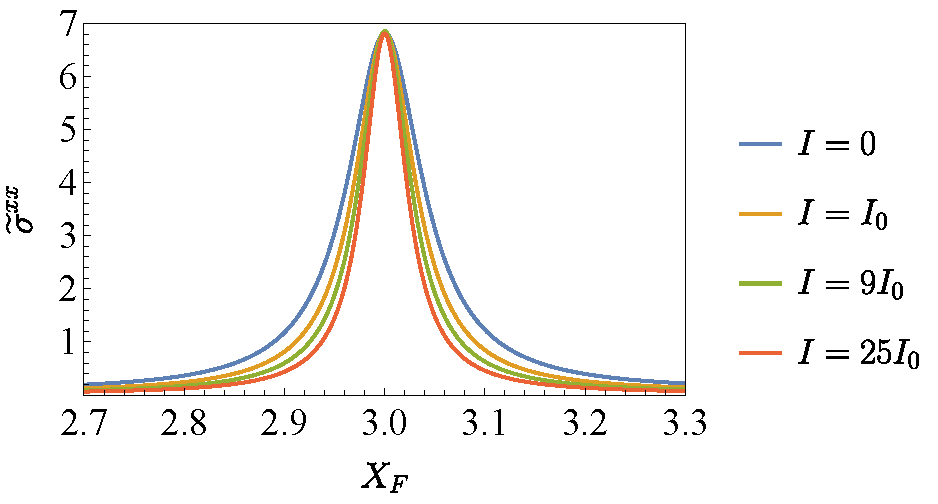
\includegraphics[scale=0.54]{fig_5_conductivity_with_fermi_level_zoomed}
\caption{$3$rd Landau level’s normalized longitudinal conductivity $\widetilde{\sigma}^{xx}$ against Fermi level $X_F$ with different intensities $I$ of the external dressing field in a GaAs-based quantum well under a nonoscillating magnetic field with $B = \SI{1.2}{\tesla}$, dressing field with a frequency of $\omega =\SI{2e12}{\radian\per\second}$ and $I_0 =\SI{100}{\watt\per\square\centi\metre}$.
In this calculation, we have assumed that the natural  broadening of $0$-th Landau level $\Gamma_0$ is $\SI{0.24}{\milli\eV}$.}
\label{fig:6}
\end{figure}
%===============================================================================

%===============================================================================
% Section 07 : Conclusions
%===============================================================================
\section{\label{sec:conclusions} Conclusions}

In this paper, we introduced a generalized mathematical model for predicting  charge transport properties in a 2DEG under a nonoscillating magnetic field and a high-intensity light. Under the uniform magnetic field, the charged particles can only settle in discrete energy values, which leads to the Landau quantization. We modeled the behavior of electrons in Landau levels under the dressing field utilizing the Floquet-Drude conductivity method. We assumed the impurities in the material as a Gaussian random scattering potential. Finally, we derived expressions for x-directional and y-directional longitudinal components of electric conductivity tensor for the considered system.

Our derived analytical expressions disclosed that we are able to control the transport characteristics of the dressed quantum Hall system by the applied dressing field’s intensity. Using detailed numerical calculations with empirical system parameters, we further analyzed the manipulation of conductivity components using the dressing field.
We found that the graphical illustrations that we obtained from these numerical calculations are capable of producing the same behavior as experiments on quantum Hall systems in the absence of a dressing field.
Furthermore, we identified that by increasing the intensity of the radiation, we can squeeze the conductivity regions near the Landau levels. Despite this behavior being identified in previous works, their results did not coincide with the more accurate description of conductivity components in undressed quantum Hall systems. However, our generalized analysis on the conductivity of dressed quantum Hall systems provide a well-suited description for these specific quantum Hall systems.

In summary, the primary purpose of this study was to broaden the modern descriptions on transport properties of dressed quantum Hall systems. Moreover, our detailed theoretical analysis showed that we can adapt the recently introduced Floquet-Drude conductivity model to extend the models that were used to describe the transport characteristics in quantum Hall systems. Owing to the ability to control the conductivity regions, high intensity external illumination may be used as a trigger for two-dimensional quantum switching devices, which are employed as the building blocks of next-generation nanoelectronic devices. As a concluding remark, we believe that our findings of this paper can be used towards understanding the 2D optoelectronic nanotransistors, enhancing their performance and inventing novel appliances.
%===============================================================================

%===============================================================================
% Acknowledgments
%===============================================================================
\begin{acknowledgments}
K.H wish to acknowledge the members of A$\chi$L at Monash University for their encouragement and support and specially T.N. Perera and R.T.Wijesekara for insightful discussions. The work of K.H is supported by the Australian Government Research Training Program (RTP) Scholarship and the Monash University Institute of Graduate Research.
\end{acknowledgments}
%===============================================================================

%===============================================================================
% Add appendixes
%===============================================================================
\appendix

%===============================================================================
% Appendix A : Wave function solutions for a dressed quantum Hall system
%===============================================================================
\section{\label{appendix_a} Wave function solutions for a dressed quantum Hall system}

The derivation of the solutions for the time-dependent Schrödinger equation with our system's Hamiltonian (Eq. \ref{eq:1}) is quite similar to that followed in Refs. \cite{husimi53,dini16}. We start with expanding the Hamiltonian for two-dimensional scenario
\begin{equation} \label{eq:a1}
  \hat{H}_e(t) = \frac{1}{2m_e}
  \left\{
    \left(\hat{p}_x + eBy \right)^2 +
    \left[
      \hat{p}_y - \frac{eE}{\omega}\cos(\omega t)
    \right]^2
  \right\}.
\end{equation}
Since $\left[\hat{H}_e(t),\hat{p}_x \right] =0$, both of these operators share same eigenfunctions
${L_x}^{-1/2}\exp(\flatfrac{ip_x x}{\hbar})$ where $p_x = \flatfrac{2\pi \hbar m}{L_x}$ with $ m \in \mathbb{Z}$.
Thus, we re-arrange the Hamiltonian using the definition of canonical momentum in $y$-direction and this leads to
\begin{equation} \label{eq:a2}
    \hat{H}_e(t) = \frac{1}{2m_e}
    \left\{
      \left({p}_x + eBy \right)^2 +
      \left[
        i\hbar \pdv{y}- \frac{eE}{\omega}\cos(\omega t)
      \right]^2
    \right\}.
\end{equation}
Subsequently, we define the \textit{center of the cyclotron orbit} on the $y$-axis as $y_0 = \flatfrac{-p_x}{(eB)}$, and the \textit{cyclotron frequency} as  $\omega_0 = {eB}/{m_e}$. This leads to a new arrangement of the Hamiltonian
\begin{equation} \label{eq:a3}
  \begin{aligned}
    \hat{H}_e(t) =
      \frac{m_e \omega_0^2}{2}\tilde{y}^2 +
      \frac{1}{2m_e} &
      \left[
        -\hbar^2 \pdv[2]{\tilde{y}}  +
        \frac{2i\hbar eE}{\omega} \cos(\omega t) \pdv{\tilde{y}}
        \right.\\
        & \left. \qquad\qquad\quad +
        \frac{e^2E^2}{\omega^2}\cos[2](\omega t)
        \right],
  \end{aligned}
\end{equation}
where we used a variable substitution $\tilde{y} = (y - y_0)$. Furthermore, we assume that the wave function solutions for the time-dependent Schrödinger equation of considered quantum system
\begin{equation} \label{eq:a4}
    i \hbar \dv{\psi}{t} = \hat{H}_e(t)\psi,
\end{equation}
can be presented by the following form
\begin{equation} \label{eq:a5}
    \psi_m(x,\tilde{y},t) = \frac{1}{\sqrt{L_x}}
    \exp\left(
      \frac{ip_x x}{\hbar} +
      \frac{ieE\tilde{y}}{\hbar \omega}\cos(\omega t)
    \right) \vartheta(\tilde{y},t),
\end{equation}
where $\vartheta(\tilde{y},t)$ is a function that satisfy the property
\begin{equation} \label{eq:a6}
    \left[
    \frac{m_e \omega_0^2}{2} \tilde{y}^2
    - {eE\tilde{y}}\sin(\omega t)
    - \frac{\hbar^2}{2m_e} \pdv[2]{\tilde{y}}
    - i \hbar \dv{t}
    \right]
    \vartheta(\tilde{y},t) = 0.
\end{equation}
If we turn off the dressing field ($E=0$), this equation leads to the Schrödinger equation with the simple harmonic oscillator Hamiltonian
\begin{equation} \label{eq:a7}
     i \hbar \dv{\vartheta(\tilde{y},t)}{t} =
    \left(
    \frac{\hat{p}_{\tilde{y}}^2}{2m_e} +
    \frac{1}{2}m_e \omega_0^2\tilde{y}^2
    \right)
    \vartheta(\tilde{y},t).
\end{equation}
Thus, we can identify $S(t) = eE\sin(\omega t)$ term as an external force that act on the harmonic oscillator, and we can solve Eq.~(\ref{eq:a6}) as a forced harmonic oscillator on $\tilde{y}$ axis
\begin{equation} \label{eq:a8}
  \begin{aligned}
    i \hbar \dv{\vartheta(\tilde{y},t)}{t} =
    \bigg[
    -
    \frac{\hbar^2}{2m_e}
    \pdv[2]{\tilde{y}} +
    \frac{1}{2}m_e \omega_0^2\tilde{y}^2
    - \tilde{y}S(t)]
    \bigg]
    \vartheta(\tilde{y},t).
  \end{aligned}
\end{equation}
This system is exactly solvable, and we can solve the equation using the methods explained by Husimi \cite{husimi53}. We introduce a time-dependent shifted coordinate $ y' = \tilde{y} - \zeta(t)$ and perform the following unitary transformation
\begin{equation} \label{eq:a9}
    \vartheta(y',t) = \exp(\frac{im_e\dot{\zeta}y'}{\hbar})\varphi(y',t).
\end{equation}
and this leads to
\begin{equation} \label{eq:a10}
  \begin{aligned}
    i \hbar \pdv{\varphi(y',t)}{t}   &=
    \left\{
        -  \frac{\hbar^2}{2m_e}\pdv[2]{{y'}}
        + \frac{1}{2} m_e \omega_0^2 y'^2
        \right. \\
        & \left. \qquad
        - \frac{1}{2} m_e\dot{\zeta}^2 + \frac{1}{2}m_e\omega_0^2 \zeta^2 - \zeta S(t)
        \right. \\
        & \left. \qquad +
        \left[
            m_e\ddot{\zeta} + m_e\omega_0^2\zeta - S(t)
        \right]y'
    \right\} \varphi(y',t).
  \end{aligned}
\end{equation}
Here, we introduced $\dot{\zeta} = \pdv*{\zeta}{t}$ and $\ddot{\zeta} = \pdv*[2]{\zeta}{t}$ for the sake of notational convenience. Subsequently, we can restrict $\zeta(t)$ function such that
\begin{equation} \label{eq:a11}
  m_e\ddot{\zeta} + m_e\omega_0^2\zeta = S(t),
\end{equation}
and that simply our previous expression as
\begin{equation} \label{eq:a12}
  \begin{aligned}
    i \hbar \pdv{\varphi(y',t)}{t} =&
    \left[
        -  \frac{\hbar^2}{2m_e}\pdv[2]{{y'}}
        + \frac{1}{2} m_e \omega_0^2 {y'}^2 \right. \\
        & \left. \qquad\qquad\qquad
        - L(\zeta,\dot{\zeta},t)
    \right]\varphi(y',t).
  \end{aligned}
\end{equation}
Here
\begin{equation} \label{eq:a13}
  L(\zeta,\dot{\zeta},t) = \frac{1}{2} m_e\dot{\zeta}^2 - \frac{1}{2}m_e\omega_0^2 \zeta^2 + \zeta S(t),
\end{equation}
is the Lagrangian of a classical driven oscillator. To proceed further, we introduce another unitary transform as follows
\begin{equation} \label{eq:a14}
    \varphi(y',t) = \exp(\frac{i}{\hbar}\int_0^{t} L(\zeta,\dot{\zeta},t')dt') \chi(y',t),
\end{equation}
and subtitling Eq.~(\ref{eq:a14}) back in Eq.~(\ref{eq:a12}), we can obtain
\begin{equation} \label{eq:a15}
    i \hbar \pdv{t} \chi(y',t)  =
    \left(
        -  \frac{\hbar^2}{2m_e}\pdv[2]{{y'}}
        + \frac{1}{2} m_e \omega_0^2 {y'}^2
    \right) \chi(y',t).
\end{equation}
This is the well-known Schrödinger equation of the quantum harmonic oscillator.
This allows us to identify the well known eigenfunction solutions \cite{griffiths18,shankar94}
\begin{equation} \label{eq:a16}
  \chi_n(y) =
  \sqrt{\frac{\kappa}{2^{n}n!\sqrt{\pi}}}
  e^{-\kappa^2 y^2/2}
  \mathcal{H}_n \qty(\kappa y),
\end{equation}
with eigenvalues
\begin{equation} \label{eq:a17}
  \epsilon_n = \hbar \omega_0 \bigg(n + \frac{1}{2}\bigg)
  ~\text{for}~
  n \in \mathbb{Z}^{+}_0.
\end{equation}
Here, $\kappa = \sqrt{{m_e \omega_0}/{\hbar}}$, and $\mathcal{H}_n$ are the Hermite polynomials.
Thus, we can identify the solutions for Eq.~(\ref{eq:a8}) as
\begin{equation} \label{eq:a18}
  \begin{aligned}
    \vartheta_n(\tilde{y},t) = \chi_n\bm{(}\tilde{y} - \zeta(t)\bm{)}
     \text{exp}&
     \left(
     \frac{i}{\hbar}
     \left\{
     - \epsilon_nt +
     m_e \left[\tilde{y}-\zeta(t)\right] \dot{\zeta(t)} \right. \right. \\
     & \left. \left. \qquad
     + \int_0^{t}L(\zeta,\dot{\zeta},t') dt'
     \right\}
     \right).
  \end{aligned}
\end{equation}
Since $\chi_n(x)$ functions forms a complete set, we can present any general solution for  $\vartheta_(\tilde{y},t)$ using the solutions derived in Eq.~(\ref{eq:a18}).

Finally, we consider our scenario where we can assume that $S(t) = eE\sin(\omega t)$, and we can derive the solution for Eq.~(\ref{eq:a11}) as
\begin{equation} \label{eq:a19}
  \zeta(t) = \frac{eE}{m_e(\omega_0^2 - \omega^2)}\sin(\omega t).
\end{equation}
Substituting solutions given in Eq.~(\ref{eq:a18}) back in Eq.~(\ref{eq:a5}), we obtain a set of wave functions with two different quantum number ($n$,$m$) that satisfy the time-dependent Schrödinger equation Eq.~(\ref{eq:a4}) as follows
\begin{equation} \label{eq:a20}
  \begin{aligned}
    &\psi_{n,m}(x,y,t) \\
    & \quad=  \frac{1}{\sqrt{L_x}}
    \chi_n\left(y - y_0 - \zeta(t)\right)\\
    &\qquad\times
    \text{exp}\left(
    \frac{i}{\hbar}
    \left\{- \epsilon_nt
    + p_x x
    + \frac{eE(y - y_0)}{\omega}\cos(\omega t) \right. \right. \\
    & \left. \left. \qquad\qquad +
    m_e\left[y - y_0 -\zeta(t)\right] \dot{\zeta}(t)+
    \int_0^{t}L(\zeta,\dot{\zeta},t') dt'
    \right\}
    \right).
  \end{aligned}
\end{equation}
%===============================================================================

%===============================================================================
% Appendix B :
%===============================================================================
\section{\label{appendix_b} Floquet modes and quasienergies}

\subsection{Position space representation}

First we define the time integral of the Lagrangian of the classical oscillator given in Eq.~(\ref{eq:5}), over a period $T=2\pi/\omega$ as
\begin{equation} \label{eq:b1}
  \Delta_{\varepsilon} = \frac{1}{T} \int_0^T L(\zeta,\dot{\zeta},t') dt'.
\end{equation}
Additionally, performing this integral, we can obtain a more simplified result
\begin{equation} \label{eq:b2}
  \Delta_{\varepsilon} = \frac{e^2E^2}{4m_e(\omega_0^2 - \omega^2)}.
\end{equation}
Next, we define another parameter
\begin{equation} \label{eq:b3}
  \xi =
  \int_0^t \; L(\zeta,\dot{\zeta},t') dt' -
  \Delta_{\varepsilon} t,
\end{equation}
and after simplifying, we can identify
\begin{equation} \label{eq:b4}
  \xi =
  \frac{e^2E^2\qty(3\omega^2 - \omega_0^2)}{8m_e\omega(\omega_0^2 - \omega^2)^2} \sin(2\omega t),
\end{equation}
which is a periodic function in time. Using these parameters, we can factorize the wave function given in Eq.~(\ref{eq:2}) as linearly time-dependent part and periodic time-dependent part as follows
\begin{equation} \label{eq:b5}
  \begin{aligned}
    \psi_{\alpha}&(x,y,t) \\
    & =
    \exp(\frac{i}{\hbar} \left(-\epsilon_nt + \Delta_{\varepsilon} t \right) )
    \frac{1}{\sqrt{L_x}} \chi_n\bm{\left(}y - y_0 - \zeta(t)\bm{\right)}
    \\
    & \quad\times
    \exp \left(
       \frac{i}{\hbar}
       \left\{
       p_x x +
       \frac{eE(y-y_0)}{\omega}\cos(\omega t)  \right. \right. \\
    & \left. \left. \qquad\qquad\qquad\qquad
    + m_e\dot{\zeta}(t) \left[ y-y_0 -\zeta(t) \right]
    + \xi \right\}
     \right).
  \end{aligned}
\end{equation}
This leads to separate the linear time-dependent phase component as the quasienergies
\begin{equation} \label{eq:b6}
  \varepsilon_{n} =
  \hbar \omega_0\qty(n + \frac{1}{2}) - \Delta_{\varepsilon},
\end{equation}
while rest of the components as time-periodic Floquet modes
\begin{equation} \label{eq:b7}
  \begin{aligned}
    \phi_{n,m}(x,y,t) =  &
    \frac{1}{\sqrt{L_x}} \chi_n\bm{\left(}y - y_0 - \zeta(t)\bm{\right)} \\
    & \times
    \exp \left(
       \frac{i}{\hbar}
       \left\{
       p_x x +
       \frac{eE(y-y_0)}{\omega}\cos(\omega t)  \right. \right. \\
    & \left. \left. \qquad\qquad\quad
    + m_e\dot{\zeta}(t) \left[ y-y_0 -\zeta(t) \right]
    + \xi \right\}
     \right).
  \end{aligned}
\end{equation}

\subsection{Momentum space representation}

We perform continuous Fourier transform over the considering confined space $A=L_xL_y$ on the Floquet modes given in Eq.~(\ref{eq:7}) to realize the Floquet modes in momentum space
\begin{equation} \label{eq:b8}
  \begin{aligned}
    \phi_{n,m}&(k_x,k_y,t) \\
    & =
    \exp(\frac{-i\gamma(t)}{\hbar}y_0)
    \exp(\frac{-i}{\hbar}\left[m_e \dot{\zeta}(t) \zeta(t) - \xi \right]) \\
    & \quad\times
    \int_{-L_y/2}^{L_y/2} \exp(-i \left[k_y - \gamma(t) \right]y)
      \chi_n \bm{\left(}y - \mu(t)\bm{\right)} dy \\
    & \quad\times
    \frac{1}{\sqrt{L_x}} \int_{-L_x/2}^{L_x/2}
     \exp(-ik_x x)\exp( \flatfrac{i p_x }{\hbar}x ) dx.
  \end{aligned}
\end{equation}
Here we used new two parameters
\begin{equation} \label{eq:b9}
  \mu(t) = \frac{eE\sin(\omega t)}{m_e(\omega_0^2 - \omega^2)} + y_0,
\end{equation}
and
\begin{equation} \label{eq:b10}
  \gamma(t) =
  \frac{eE\omega_0^2\cos(\omega t)}{\hbar\omega(\omega_0^2 - \omega^2)}.
\end{equation}
Subsequently, using the Fourier transform identity \cite{bruus04}
\begin{equation} \label{eq:b11}
  \int_{-L_x/2}^{L_x/2}
  \exp( -ik_x x + \flatfrac{i p_x x}{\hbar}) dx =
  L_x \delta_{k_x,\flatfrac{p_x}{\hbar}},
\end{equation}
we can derive
\begin{equation} \label{eq:b12}
  \begin{aligned}
    \phi_{n,m}(k_x,k_y,t)  =
    \Phi_{n,m}&(k_y,t)
    \delta_{k_x,\flatfrac{p_x}{\hbar}}
    \exp(\frac{-i}{\hbar} \gamma(t)y_0) \\
    & \times
    \exp(\frac{-i}{\hbar}
    \left[ m_e \dot{\zeta}(t) \zeta(t) - \xi \right]),
  \end{aligned}
\end{equation}
where we can define $\Phi_{n,m}(k_y,t)$ as
\begin{equation} \label{eq:b13}
  \begin{aligned}
    &\Phi_{n,m}(k_y,t) \\
    & \quad=
    \sqrt{L_x}
    \int_{-L_y/2}^{L_y/2}
    \chi_n \bm{\left(}y - \mu(t)\bm{\right)}
    \exp \bm{\left(}-i\left[k_y - \gamma(t) \right]y\bm{\right)} dy.
  \end{aligned}
\end{equation}
Substituting ${k'_y} = k_y -\gamma(t)$ with $y' = y -\mu(t)$, and assuming that the size of the considered 2DEG sample in $y$-direction is considerably large ($L_y \rightarrow \infty$), we can obtain
\begin{equation} \label{eq:b14}
  \Phi_{n,m}({k'_y} ,t) =
  {\sqrt{L_x}} e^{-i {k'_y}\mu}
  \int_{-\infty}^{\infty} \chi_{n}(y') \exp(-i{k'_y} y') dy'.
\end{equation}
Moreover, we can identify that the above integral represents the Fourier transform of $\chi_n$ functions. In addition, using the symmetric conditions of the Fourier transform for Gauss-Hermite functions $\theta_n(x)$ \cite{celeghini21}
\begin{equation} \label{eq:b15}
  \mathcal{FT}[\theta_n(\kappa x),x,k] = \frac{i^n}{|\kappa|}\theta_n(k/\kappa),
\end{equation}
we can simply the Eq.~(\ref{eq:b14}) as
\begin{equation} \label{eq:b16}
  \Phi_{n,m}({k'_y} ,t) =
  \sqrt{L_x} e^{-i {k'_y}\mu} \widetilde{\chi}_n(k'_y),
\end{equation}
with
\begin{equation} \label{eq:b17}
  \widetilde{\chi}_{n}(k) =
  \frac{i^n}{\sqrt{2^{n} n! \sqrt{\pi}}}
  \left(\frac{1}{\kappa} \right)^{1/2}
  e^{-\flatfrac{k^2}{(2 \kappa^2)}}
  \mathcal{H}_n (\flatfrac{k}{\kappa}).
\end{equation}
Finally, substitute Eq.~(\ref{eq:b16}) back into Eq.~(\ref{eq:b12}) and this leads to
\begin{equation} \label{eq:b18}
  \begin{aligned}
    \phi_{n,m}(k_x,k_y,t)  = &
    {\sqrt{L_x}} \widetilde{\chi}_n \bm{\left(} k_y - b\cos(\omega t)\bm{\right)} \\
    & \times
    \exp \left(
      i\xi -ik_y  \left[d\sin(\omega t) + \frac{\hbar k_x}{eB} \right]
    \right),
  \end{aligned}
\end{equation}
where
\begin{equation} \label{eq:b19}
  b =
  \frac{eE\omega_0^2}{\hbar\omega(\omega_0^2 - \omega^2)},
\end{equation}
and
\begin{equation} \label{eq:b20}
  d =
 \frac{eE}{m_e(\omega_0^2 - \omega^2)}.
\end{equation}
It is necessary to notice that $k_x$ is quantized with $k_x = \flatfrac{2\pi m}{L_x} ~,~ m \in \mathbb{Z}$.
%===============================================================================

%===============================================================================
% Appendix C :
%===============================================================================
\section{\label{appendix_c} Floquet-Fermi golden rule for a dressed quantum  Hall system}

We derive the Floquet-Fermi golden rule for our dressed quantum Hall system with the help of the $t$-$t'$ formalism. The $t$-$t'$-Floquet states \cite{grifoni98,wackerl20}
\begin{equation} \label{eq:c1}
  \ket{\psi_{n,m}(t,t')} =
  \exp(-\frac{i}{\hbar}\varepsilon_{n} t)\ket{\phi_{n,m}(t')},
\end{equation}
are derived by separating the aperiodic and periodic components of the Floquet states given in Eq.~(\ref{eq:14}). Additionally, these states fulfill the $t$-$t'$-Schrödinger equation \cite{grifoni98,wackerl20}
\begin{equation} \label{eq:c2}
  i \hbar \pdv{t}\ket{\psi_{n,m}(t,t')} =
  H_F(t') \ket{\psi_{n,m}(t,t')},
\end{equation}
where the \textit{Floquet Hamiltonian} defined as
\begin{equation} \label{eq:c3}
  H_F(t') =
  H_e(t') - i\hbar \pdv{t'}.
\end{equation}
Next, we can identify the time evolution operator corresponding to the $t$-$t'$-Schrödinger equation as
\begin{equation} \label{eq:c4}
  U_F(t,t_0;t') = \exp(-\frac{i}{\hbar}H_F(t')\left[t-t_0 \right]).
\end{equation}
The advantage of $t$-$t'$ formalism lies on this time evolution operator which avoids any time ordering operators \cite{wackerl20}.

We model the effect caused by impurities in the considered system as a single perturbation potential formed by a group of randomly distributed impurities.
Thus, we introduce a time-independent total perturbation $V(\vb{r})$ which has been turned on at the reference time $t=t_0$, and the $t$-$t'$-Schrödinger equation becomes
\begin{equation} \label{eq:c5}
  i \hbar \pdv{t}\ket{\Psi_{n,m}(t,t')} =
  \left[H_F(t') + V(\vb{r}) \right]\ket{\Psi_{n,m}(t,t')}.
\end{equation}
This introduces a new wave function solution $\ket{\Psi_{n,m}}$ for a system with a given perturbation. If $t\leq t_0$, both of the solutions for Eq.~(\ref{eq:c2}) and Eq.~(\ref{eq:c5}) coincide
\begin{equation} \label{eq:c6}
  \ket{\psi_{n,m}(t,t')} =\ket{\Psi_{n,m}(t,t')} \quad
  \text{when} \quad
  t \leq t_0.
\end{equation}
Next, we move our analysis into the interaction picture representation \cite{bruus04,mahan00} and in the interaction picture, we can identify the $t$-$t'$-Floquet state as
\begin{equation} \label{eq:c7}
  \ket{\Psi_{n,m}(t,t')}_I = U_0^{\dagger}(t,t_0;t')
  \ket{\Psi_{n,m}(t,t')}.
\end{equation}
Due to time-independence, the perturbation in the interaction picture has the same form as the Schrödinger picture representation
\begin{equation} \label{eq:c8}
  V_I(\vb{r}) = U_0^{\dagger}(t,t_0;t')V(\vb{r})U_0(t,t_0;t') =
  V(\vb{r}).
\end{equation}
This leads us to the $t$-$t'$-Schrödinger equation in the interaction picture representation
\begin{equation} \label{eq:c9}
  i \hbar \pdv{t}\ket{\Psi_{n,m}(t,t')}_I =
  V_I(\vb{r})\ket{\Psi_{n,m}(t,t')}_I,
\end{equation}
with the recursive solutions \cite{bruus04,mahan00}
\begin{equation} \label{eq:c10}
  \begin{aligned}
  \ket{\Psi_{n,m}(t,t')}_I = &\ket{\Psi_{n,m}(t_0,t')}_I \\
  &+
  \frac{1}{i\hbar}
  \int_{t_0}^t
  V_I(\vb{r}) \ket{\Psi_{n,m}(t_1,t')}_I dt_1.
  \end{aligned}
\end{equation}
Iterating the solution only up to the first order (Born approximation) we obtain
\begin{equation} \label{eq:c11}
  \begin{aligned}
    \ket{\Psi_{n,m}(t,t')}_I \approx &\ket{\psi_{n,m}(t_0,t')} \\
    &+
    \frac{1}{i\hbar}
    \int_{t_0}^t
    V_I(\vb{r}) \ket{\psi_{n,m}(t_0,t')} dt_1.
  \end{aligned}
\end{equation}

Since our $t$-$t'$-Floquet states create a basis, we can represent the solutions for the $t$-$t'$-Schrödinger equation given in Eq.~(\ref{eq:c5}) using our known $t$-$t'$-Floquet states as follows
\begin{equation} \label{eq:c12}
  \ket{\Psi_{\alpha}(t,t')} = \sum_{\beta} a_{\alpha,\beta}(t,t')
  \ket{\psi_{\beta}(t,t')}.
\end{equation}
Here, we used a single term notation to represent two quantum numbers; $\alpha \equiv (n_{\alpha},m_{\alpha})$ and $\beta \equiv (n_{\beta},m_{\beta})$.
Subsequently, we can identify the \textit{scattering amplitude} as $a_{\alpha,\beta}(t,t') =
\braket{\psi_{\beta}(t,t')}{\Psi_{\alpha}(t,t')}$ and we can evaluate this with
\begin{equation} \label{eq:c13}
  \begin{aligned}
  a_{\alpha,\beta}(t,t') = &
  \braket{\psi_{\beta}(t,t')}{\psi_{\alpha}(t,t')} \\
  &+
  \frac{1}{i\hbar}
  \int_{t_0}^t
  \bra{\psi_{\beta}(t_1,t')}
  V(\vb{r}) \ket{\psi_{\alpha}(t_1,t')} dt_1.
  \end{aligned}
\end{equation}
Since the $t$-$t'$-Floquet states are orthonormal and assuming $t_0 = 0$ and $\alpha \neq \beta$ this leads to
\begin{equation} \label{eq:c14}
  a_{\alpha,\beta}(t,t') =
  -
  \frac{i}{\hbar}
  \int_{0}^t
  \bra{\psi_{\beta}(t_1,t')}
  V(\vb{r}) \ket{\psi_{\alpha}(t_1,t')} dt_1.
\end{equation}

Next, we consider a scattering phenomenon when a electron scatters from a known $t$-$t'$-Floquet state $\ket{\psi_{\beta}(t,t')} $ into a distinct $t$-$t'$-Floquet state $\ket{\Psi_{\alpha}(t,t')}$ with a constant quansienergy $\varepsilon$ as follows
\begin{equation} \label{eq:c15}
  \begin{aligned}
  \ket{\psi_{\beta}(t,t')} &= \exp(-\frac{i}{\hbar}\varepsilon_{\beta} t)
  \ket{\phi_{\beta}(t')} \\
  &
  \xRightarrow{\text{scattering}}
  \ket{\Psi_{\alpha}(t,t')} = \exp(-\frac{i}{\hbar}\varepsilon t)
  \ket{\Phi_{\alpha}(t')}.
  \end{aligned}
\end{equation}
\begin{figure}[b]
  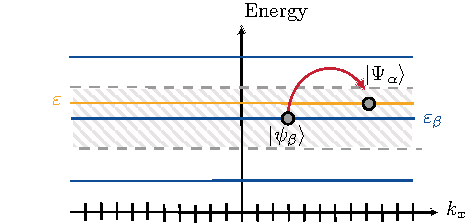
\includegraphics[scale=1.0]{fig_6_scattering_scenario.pdf}
  \caption{Scattering from known $\ket{\psi_{\beta}(t,t')}$ state to a constant energy state $\ket{\Psi_{\alpha}(t,t')}$ due to the scattering potential created by impurities in the material.}
  \label{fig:2}
\end{figure}
This phenomenon is illustrated in Fig.~\ref{fig:2}.
We can calculate the scattering amplitude for this scattering scenario using the expression derived in Eq.~(\ref{eq:c14}) as follows
\begin{equation} \label{eq:c16}
  \begin{aligned}
    a_{\alpha\beta}(t,t') =
    -\frac{i}{\hbar}
    \int_{0}^t
    e^{\frac{i}{\hbar}\left(\varepsilon_{\beta} - \varepsilon \right)t_1}
    \bra{\phi_{\beta}(t')}
    V(\vb{r}) \ket{\phi_{\alpha}(t')}  dt_1.
  \end{aligned}
\end{equation}
By assuming for a long duration ($t \rightarrow \infty$), we can turn this integral into a delta distribution
\begin{equation} \label{eq:c17}
  \begin{aligned}
    a_{\alpha\beta}(t') =
    -2\pi i \delta(\varepsilon_{\beta} - \varepsilon)Q,
  \end{aligned}
\end{equation}
where $Q = \bra{\phi_{\beta}(t')} V(\vb{r}) \ket{\phi_{\alpha}(t')}$ and using the completeness properties we can re-write this as
\begin{equation} \label{eq:c18}
    Q =
    \sum_{\vb{k}}\sum_{\vb{k'}}
    \braket{\phi_{\beta}(t')}{\vb{k'}}
    \mel{\vb{k'}}{V(\vb{r})}{\vb{k}}
    \braket{\vb{k}}{\phi_{\alpha}(t')}.
\end{equation}
Moreover, separating $x$-directional and $y$-directional momentum components, we can simply this to obtain
\begin{equation} \label{eq:c19}
    Q =
    \sum_{k_x}\sum_{{k'}_x}
    \int_{-\infty}^{\infty} \int_{-\infty}^{\infty}
    V_{\vb{k'},\vb{k}}
    \phi_{\beta}^{\dagger}(\vb{k'},t')
    \phi_{\alpha}(\vb{k},t')  dk_y d{k'}_y,
\end{equation}
with $V_{\vb{k'},\vb{k}} = \mel{\vb{k'}}{V(\vb{r})}{\vb{k}}$.

Since we are presenting the the perturbation potential $V(\vb{r})$ by a group of randomly distributed impurities, we take into account $N_{imp}$ number of identical single impurity potentials distributed at randomly but in fixed positions $\vb{r}_i$. Thus, we can describe the scattering potential $V(\vb{r})$ as the sum of uncorrelated single impurity potentials $\upsilon(\vb{r})$
\begin{equation} \label{eq:c20}
  V(\vb{r}) =
  \sum_{i=1}^{N_{imp}}
  \upsilon (\vb{r}-\vb{r}_i).
\end{equation}
Furthermore, we model the perturbation $V(\vb{r})$ as a Gaussian random potential where one can choose the zero of energy such that the potential is zero on average. This model is characterized by the following two equations \cite{akkermans10}
\begin{subequations}
\begin{equation} \label{eq:c21a}
  \expval{\upsilon(\vb{r})}_{imp} =0,
\end{equation}
\begin{equation} \label{eq:c21b}
  \expval{\upsilon(\vb{r})\upsilon(\vb{r'})}_{imp} = \Upsilon(\vb{r}-\vb{r'}),
\end{equation}
\end{subequations}
where $\expval{\cdot}_{imp}$ represents the average over the impurity disorder and $\Upsilon(\vb{r}-\vb{r'})$ is any decaying function depends only on $\vb{r}-\vb{r'}$. In addition, this model assumes that $\upsilon (\vb{r}-\vb{r'})$ only depends on the magnitude of the position difference $|\vb{r}-\vb{r'}|$, and it decays with a characteristic length $r_c$. Since this study considers the case where the wavelength of radiation or scattering electron is much greater than $r_c$, it is a better approximation to make two-point correlation function to be
\begin{equation} \label{eq:c22}
  \expval{\upsilon(\vb{r})\upsilon(\vb{r'})}_{imp} = \Upsilon_{imp}^2\delta(\vb{r}-\vb{r'}),
\end{equation}
where $\Upsilon_{imp}^2$ is a constant. A random potential $V(\vb{r})$ with this property is called white noise \cite{akkermans10}. Then we can approximately model the total scattering potential as
\begin{equation} \label{eq:c23}
  V(\vb{r}) =
  \sum_{i=1}^{N_{imp}}
  \Upsilon_{imp} \delta(\vb{r}-\vb{r}_i).
\end{equation}
Here we can identify the $\Upsilon_{imp}$ as the strength of the delta potential.
Furthermore, we can calculate $V_{\vb{k'},\vb{k}}$ using this assumption as follows
\begin{subequations} \label{eq:c24}
\begin{align}
 V_{\vb{k'},\vb{k}} & =
 \mel**{\vb{k'}}{\sum_{i=1}^{N_{imp}}
 \Upsilon_{imp} \delta(\vb{r}-\vb{r}_i)}{\vb{k}} \label{eq:c24a} \\
 & =
 \sum_{i=1}^{N_{imp}}
 \int_{-\infty}^{\infty} \left[
 \frac{1}{\sqrt{L_xL_y}} e^{ik'_y y} \delta(y-y_i) \nonumber \right. \\
 & \left. \qquad\quad\times
 \frac{1}{\sqrt{L_xL_y}} e^{-i{k}_y y}
 \mel**{k'_x}{\Upsilon_{imp} \delta(x-x_i)}{k_x} \right] dy \label{eq:c24b} \\
  & =
 \sum_{i=1}^{N_{imp}} \frac{1}{{L_xL_y}}
 e^{i(k'_y - k_y )y}
 \mel**{k'_x}{\Upsilon_{imp} \delta(x-x_i)}{k_x} \label{eq:c24c}.
\end{align}
\end{subequations}
Since $\upsilon (\vb{r})$ in momentum space is a constant value, each impurity  produce same impurity potential for every $x$-directional momentum pairs. Additionally, assuming the total number of scatters $N_{imp}$ is microscopically large, we can derive
\begin{subequations} \label{eq:c25}
  \begin{align}
    V_{\vb{k'},\vb{k}}
    & =
    V_{k'_x,k_x}
    \frac{N_{imp}}{L_y L_x} \int_{-\infty}^{\infty}
    e^{i\left({k'}_y - k_y \right)y_i} dy_i \label{eq:c25a} \\
    & =
    \eta_{imp} V_{k'_x,k_x} \delta(k'_y - k_y). \label{eq:c25b}
  \end{align}
\end{subequations}
In the above equation we introduced
\begin{equation} \label{eq:c26}
  V_{{k'}_x,k_x} =
  \mel**{k'_x}{\Upsilon_{imp} \delta(x-x_i)}{k_x},
\end{equation}
which is a constant value for every $i$-th impurity. Moreover, $\eta_{imp}$ is the number of impurities in a unit area. It is important to note that in the above expression $\braket{x}{k_x} = e^{-ik_xx}$.

Now using Eq.~(\ref{eq:10}) and Eq.~(\ref{eq:c25b}) on Eq.~(\ref{eq:c19}), we obtain
\begin{equation} \label{eq:c27}
  \begin{aligned}
    Q  =
    \sum_{k_x}\sum_{{k'}_x} &
    {\eta_{imp} V_{{k'}_x,k_x}} L_x
    \int_{-\infty}^{\infty} \int_{-\infty}^{\infty}
    \delta({k'}_y - k_y)
    \\
    & \times
    \widetilde{\chi}_{n_{\beta}} \bm{\left(} {k'}_y -b\cos(\omega t) \bm{\right)}
    \widetilde{\chi}_{n_{\alpha}}  \bm{\left(}k_y -b\cos(\omega t) \bm{\right)}
    \\
    & \times
    e^{i[{k'}_y - k_y]d\sin(\omega t)}
    e^{i[{k'}_y {y'}_0 - k_y y_0]}
     dk'_y dk_y.
  \end{aligned}
\end{equation}
Here we have changed the time variable $t' \rightarrow t$ only for the simplicity of notation. We can more simply this as
\begin{equation} \label{eq:c28}
  \begin{aligned}
    Q =
    \sum_{k_x}\sum_{{k'}_x} \eta_{imp} L_x V_{{k'}_x,k_x} I,
  \end{aligned}
\end{equation}
with
\begin{equation} \label{eq:c29}
  \begin{aligned}
    I =
    \int_{-\infty}^{\infty}
    \widetilde{\chi}_{n_{\beta}} &\bm{\left(}  k_y -b\cos(\omega t) \bm{\right)}
    \widetilde{\chi}_{n_{\alpha}} \bm{\left(} k_y -b\cos(\omega t) \bm{\right)} \\
    & \times
    \exp \bm{(}
      -ik_y  \left(y_0 - {y'}_0 \right)
    \bm{)} dk_y.
  \end{aligned}
\end{equation}
To avoid the energy exchange from the dressing field and electrons in Landau levels, the applied radiation must be a purely dressing field.
Therefore, in this study we assume that the dressing field can only renormalize the the probability of electron scattering inside a same Landau energy level $(n_{\alpha} = n_{\beta} =N)$. This transform the Eq.~(\ref{eq:c29}) to
\begin{equation} \label{eq:c30}
    I =
    \int_{-\infty}^{\infty}
    \widetilde{\chi}_N^2 \bm{\left(}  k_y -b\cos(\omega t) \bm{\right)}
    \exp \bm{(}
      -ik_y  \left(y_0 - {y'}_0 \right)
    \bm{)} dk_y.
\end{equation}
Using the Fourier transform of Gauss-Hermite functions \cite{celeghini21} and the convolution theorem \cite{arfken85,bracewell78} we obtain
\begin{equation} \label{eq:c31}
  \begin{aligned}
    I =
    {2\pi} &
    \exp \bm{(} b({y'}_0 - y_0)\cos(\omega t) \bm{)} \\
    & \times
    \int_{-\infty}^{\infty}
    {\chi}_{N}(y)
    {\chi}_{N}(y_0 - {y'}_0 - y) dy.
  \end{aligned}
\end{equation}
Finally, we can evaluate the scattering amplitude derived in Eq.~(\ref{eq:c17}) for given $k_x = 2\pi m_{\alpha}/L_x$ and $k'_x =  2\pi m_{\beta}/L_x$ as follows
\begin{equation} \label{eq:c32}
  \begin{aligned}
    a_{\alpha\beta}&(k_x,k'_x,t)
    \\
    & =
    -2\pi i
    \eta_{imp} L_x V_{{k'}_x,k_x}
    e^{ b({y'}_0 - y_0)\cos(\omega t)}\\
    & \quad\times
    \delta(\varepsilon_{N} - \varepsilon)
    \int_{-\infty}^{\infty}
    {\chi}_{N}(y)
    {\chi}_{N}(y_0 - {y'}_0 - y) dy.
  \end{aligned}
\end{equation}
Since this scattering amplitude is time-periodic, we can write this as a Fourier series expansion
\begin{equation} \label{eq:c33}
    a_{\alpha\beta}(k_x,k'_x,t) =
    \sum_{l=-\infty}^{\infty} a^l_{\alpha\beta}(k_x,k'_x) e^{-il\omega t}.
\end{equation}
In addition, using Jacobi-Anger expansion \cite{cuyt08,abramowitz64}
\begin{equation} \label{eq:c34}
    e^{iz\cos(\theta)} = \sum_{l=-\infty}^{\infty} i^l J_l(z) e^{-il\theta},
\end{equation}
where $J_l(\cdot)$ are Bessel functions of the first kind with $l$-th integer order, we can re-write the Eq.~(\ref{eq:c32}) as follows
\begin{equation} \label{eq:c35}
  \begin{aligned}
    a_{\alpha\beta}&(k_x,k'_x,t)  \\
    & =
    \sum_{l=-\infty}^{\infty}
    -2\pi i^{l+1}
    \eta_{imp} L_x V_{{k'}_x,k_x}
    J_l\bm{(}b({y'}_0 - y_0)\bm{)} \\
    & \quad\times
    \delta(\varepsilon_{N} - \varepsilon)
    \int_{-\infty}^{\infty}
    {\chi}_{N}(y)
    {\chi}_{N}(y_0 - {y'}_0 - y)  dy \;e^{-il\omega t}.
  \end{aligned}
\end{equation}
Thus, we can identify the Fourier series component of the scattering amplitude as
\begin{equation} \label{eq:c36}
  \begin{aligned}
    a^l_{\alpha\beta}(k_x,k'_x) = &
    -2\pi i^{l+1}
    \eta_{imp} L_x V_{{k'}_x,k_x}\\
    & \times
    \delta(\varepsilon_{N} - \varepsilon)
    J_l\bm{(}b({y'}_0 - y_0)\bm{)}\\
    & \times
    \int_{-\infty}^{\infty}
    {\chi}_N(y)
    {\chi}_N(y_0 - {y'}_0 - y) dy.
  \end{aligned}
\end{equation}
Furthermore, we can define \textit{transition probability matrix} as
\begin{equation} \label{eq:c37}
    \left(A_{\alpha\beta} \right)^{l,l'} =
    a^l_{\alpha\beta}\left[a^{l'}_{\alpha\beta} \right]^{*},
\end{equation}
and this becomes
\begin{equation} \label{eq:c38}
  \begin{aligned}
      \left(A_{\alpha\beta} \right)^{l,l'}(k_x,k'_x) = &
      \left({ 2 \pi \eta_{imp} L_x V_{{k'}_x,k_x}}\right)^2
      \delta^2(\varepsilon_{N} - \varepsilon) \\
      & \times
      J_l\bm{(}b({y'}_0 - y_0)\bm{)} J_{l'}\bm{(}b({y'}_0 - y_0)\bm{)}\\
      & \times
      \left|
      \int_{-\infty}^{\infty}
      {\chi}_N(y)
      {\chi}_N(y_0 - {y'}_0 - y) dy \right|^2.
  \end{aligned}
\end{equation}
Then describing the square of the delta distribution using the following interpretation \cite{dini16,kibis14}
\begin{equation} \label{eq:c39}
    \delta^2(\varepsilon) =
    \delta(\varepsilon)\delta(0) =
    \frac{\delta(\varepsilon)}{2\pi \hbar}
    \int_{-t/2}^{t/2} e^{i0\times t'/\hbar} dt'\; =
    \frac{\delta(\varepsilon)t}{2\pi \hbar},
\end{equation}
and executing the time derivation operation on each matrix element of transition probability matrix, we receive the \textit{transition amplitude matrix} elements
\begin{equation} \label{eq:40}
  \begin{aligned}
    \Gamma_{\alpha\beta}^{ll'}(k_x,k'_x) = &
    \frac { 2\pi \eta_{imp}^2 L_x^2}{ \hbar} |V_{{k'}_x,k_x}|^2
    \delta(\varepsilon_{\beta} - \varepsilon)\\
    & \times
    J_l\bm{(}b({y'}_0 - y_0)\bm{)} J_{l'}\bm{(}b({y'}_0 - y_0)\bm{)} \\
    & \times
    \left|
    \int_{-\infty}^{\infty}
    {\chi}_N(y)
    {\chi}_N(y_0 - {y'}_0 - y) dy \right|^2.
  \end{aligned}
\end{equation}

Additionally, the inverse scattering time matrix can be identified as the sum of all available momentum over the impurity averaged transition probability matrix element \cite{wackerl20,wackerlthesis20}
\begin{equation} \label{eq:41}
    \left(\frac{1}{\tau(\varepsilon,k_x)} \right)^{ll'}_{\alpha\beta} =
    \frac{1}{L_x} \sum_{{k'}_x}
    \expval**{\Gamma_{\alpha\beta}^{ll'}({k'}_x,k_x)}_{imp}.
\end{equation}
Next, applying the 1-dimensional momentum continuum limit $\sum_{{k'}_x} \longrightarrow {L_x}/{2\pi}\int d {k'}_x$, we can obtain
\begin{widetext}
\begin{equation} \label{eq:42}
  \begin{aligned}
    \left(\frac{1}{\tau(\varepsilon,k_x)}\right)^{ll'}_{\alpha\beta} = &
    \frac { 2\pi \eta_{imp}^2 L_x^2}{ \hbar}
    \frac{V_{imp}}{2\pi}
    \delta(\varepsilon_{\beta} - \varepsilon) \\
    & \times
    \int_{-\infty}^{\infty} \left\{
    J_l\bm{\left(}\frac{b\hbar}{eB}({k}_x - {k'}_x)\bm{\right)}
    J_{l'}\bm{\left(}\frac{b\hbar}{eB}({k}_x - {k'}_x)\bm{\right)}
    \left|
    \int_{-\infty}^{\infty}
    {\chi}_N(y)
    {\chi}_N \bm{\left(}\frac{\hbar}{eB} ({k'}_x - {k}_x) - y \bm{\right)} dy\right|^2 \right\} d {k'}_x.
  \end{aligned}
\end{equation}
Here an impurity average of white noise potential allows to identify $\expval{|V_{{k'}_x,k_x}|^2}_{imp} = V_{imp}$.
Finally, using substitutions $k'_x = k_1$ and $y = \flatfrac{\hbar{k_2}}{(eB)}$, we can derive our expression for the inverse scattering time matrix for $N$-th Landau
level as follows
\begin{equation} \label{eq:43}
  \begin{aligned}
    \left(\frac{1}{\tau(\varepsilon,k_x)}\right)^{ll'}_{N} &=
    \frac { \eta_{imp}^2 L_x^2 \hbar V_{imp}}{e^2B^2}
    \delta(\varepsilon - \varepsilon_{N}) \\
    & \times
    \int_{-\infty}^{\infty} \left\{
    J_l\bm{\left(}\frac{b\hbar}{eB}({k}_x - k_1)\bm{\right)}
    J_{l'}\bm{\left(}\frac{b\hbar}{eB}({k}_x - k_1)\bm{\right)}
    \left|
    \int_{-\infty}^{\infty}
    {\chi}_N\left(\frac{\hbar}{eB}k_2 \right)
    {\chi}_N \bm{\left(}\frac{\hbar}{eB} (k_1 - k_x - k_2) \bm{\right)} dk_2 \right|^2 \right\} d k_1.
  \end{aligned}
\end{equation}
\end{widetext}
%===============================================================================

%===============================================================================
% Appendix D :
%===============================================================================
\section{\label{appendix_d} Current operators for a dressed quantum Hall system}

In this section, we derive the current density operator for the $N$-th Landau level in a dressed quantum Hall system. We already found the exact solution for the time-dependent Schrödinger equation with the Hamiltonian give in Eq.~(\ref{eq:1}) and we identified them as the Floquet states in Eq.~(\ref{eq:14}). For the simplicity of notation, we can represent the Floquet modes derived in Eq.~(\ref{eq:10}) as quantum states using their corresponding quantum numbers as follows
\begin{equation} \label{eq:d1}
  \ket{\phi_{n,m}} = \ket{n,k_x}.
\end{equation}
Using this complete set of quantum states \cite{wackerl20,holthaus15,grifoni98}, we can represent the single particle current operator's matrix element as
\begin{equation} \label{eq:d2}
  \left(\vb{j} \right)_{nm,n'm'} = \mel{n,k_x}{\;\hat{\vb{j}}\;}{n',k'_x}.
\end{equation}
Next, we can identify the particle current operator for our system \cite{mahan00,bruus04} as
\begin{equation} \label{eq:d3}
  \hat{\vb{j}} = \frac{1}{\widetilde{m}} \left\{\hat{\vb{p}} - e\left[\vb{A}_s + \vb{A}_d(t) \right]\right\},
\end{equation}
where $\widetilde{m}$ is the mass of the considering particle.

First, we consider the $x$-directional particle current operator component, and we can identify that as
\begin{equation} \label{eq:d4}
  \hat{j}_x = \frac{1}{\widetilde{m}} \left(-i\hbar\pdv{x} + eBy \right).
\end{equation}
Next, we calculate the matrix elements of $x$-directional current operator against our Floquet mode basis
\begin{equation} \label{eq:d5}
  \left({j}_x \right)_{nm,n'm'} =
  \mel{n,k_x}{\;\frac{1}{\widetilde{m}} \left(-i\hbar\pdv{x} + eBy \right)}{n',k'_x},
\end{equation}
and we evaluate these using the Floquet modes derived in Eq.~(\ref{eq:7}) as follows
\begin{equation} \label{eq:d6}
  \begin{aligned}
    \left({j}_x \right)_{nm,n'm'} = &
    \frac{1}{{\widetilde{m}}}
    \delta_{k_x,k'_x}
    \int
    \left(\hbar k'_x + eBy\right) \\
    & \times
     \chi_{n}\bm{\left(}y - y_0 - \zeta(t)\bm{\right)}
    \chi_{n'}\bm{\left(}y - y_0 - \zeta(t)\bm{\right)}
    dy.
  \end{aligned}
\end{equation}
Let $[y - y_0 - \zeta(t)] = \bar{y}$ and we can obtain
\begin{equation} \label{eq:d7}
  \begin{aligned}
    \left({j}_x \right)_{nm,n'm'} =
    \frac{1}{{\widetilde{m}}}
    \delta_{k_x,k'_x}
    \int &
    \left[ \hbar k'_x + eB\bar{y} -\hbar k'_x + eB\zeta(t)\right] \\
    & \times
    \chi_{n}(\bar{y})
    \chi_{n'}(\bar{y})
    d\bar{y}.
  \end{aligned}
\end{equation}
Using the following integral identities of the Floquet modes which are made up with Gauss-Hermite functions \cite{vedenyapin11,szego59}
\begin{subequations} \label{eq:d8}
  \begin{align}
    \int
    \chi_{n}({y})
    \chi_{n'}({y}) d{y} &=
    \delta_{n',n}, \\
    \int
    y \chi_{n}({y})\chi_{n'}({y}) d{y} &=
    \left(\sqrt{\frac{n+1}{2}} \delta_{n',n+1} + \sqrt{\frac{n}{2}}
    \delta_{n',n-1} \right),
  \end{align}
\end{subequations}
we simplify the matrix elements of $x$-directional current operator to obtain
\begin{equation} \label{eq:d9}
  \begin{aligned}
    &\left({j}_x \right)_{nm,n'm'} =
    \frac{eB}{{\widetilde{m}}}
    \delta_{k_x,k'_x} \\
    & \qquad\times
    \left[
    \left(\sqrt{\frac{n+1}{2}} \delta_{n',n+1} + \sqrt{\frac{n}{2}}
    \delta_{n',n-1}\right)
    + \zeta(t) \delta_{n',n}
    \right].
  \end{aligned}
\end{equation}
Due to high complexity of extract solution, in this study we only consider the constant contribution. Therefore, we can identify the $0$-th component of the Fourier series as
\begin{equation} \label{eq:d10}
  \begin{aligned}
      \left({j}_x \right)_{nm,n'm'} =&
      \frac{eB}{\widetilde{m}}
      \delta_{k_x,k'_x} \\
      & \times
      \left(\sqrt{\frac{n+1}{2}} \delta_{n',n+1} + \sqrt{\frac{n}{2}}
      \delta_{n',n-1} \right).
  \end{aligned}
\end{equation}
For a electric current operator, we can apply the electron's charge and the  effective mass of the electron to the above derived equation. This leads to
\begin{equation} \label{eq:d11}
  \begin{aligned}
      \Big({j}^x_{s=0}\Big)_{nm,n'm'}^{electron}  =&
      \frac{e^2B}{{m_e}}
      \delta_{k_x,k'_x}\\
      & \times
      \left(\sqrt{\frac{n+1}{2}} \delta_{n',n+1} + \sqrt{\frac{n}{2}}
      \delta_{n',n-1} \right).
  \end{aligned}
\end{equation}

Moreover, we can identify the $y$-directional current operator component as
\begin{equation} \label{eq:d12}
  \hat{j}_y = \frac{1}{\widetilde{m}} \left(-i\hbar\pdv{y} - \frac{eE}{\omega}\cos(\omega t) \right).
\end{equation}
Using this operator, we can represent the matrix elements of $y$-directional current operator in Floquet mode basis as
\begin{equation} \label{eq:d13}
  \left({j}_y \right)_{nm,n'm'} =
  \mel{n,k_x}{\;\frac{-1}{\widetilde{m}} \left(i\hbar\pdv{y} + \frac{eE}{\omega}\cos(\omega t) \right)}{n',k'_x}.
\end{equation}
After following the same steps done for the $x$-directional current operator, we can identify the $0$-th component of matrix elements for $y$-directional electric current operator as
\begin{equation} \label{eq:d14}
  \begin{aligned}
    \Big({j}^y_{s=0}\Big)_{nm,n'm'}^{electron} = &
    \frac{ie\hbar}{{m_e}}
    \delta_{k_x,k'_x} \\
    & \times
    \left(
    \sqrt{\frac{n}{2}} \delta_{n',n-1}
    - \sqrt{\frac{n+1}{2}} \delta_{n',n+1}
    \right).
  \end{aligned}
\end{equation}
%===============================================================================

%===============================================================================
% Bibliography
%===============================================================================
%apsrev4-2.bst 2019-01-14 (MD) hand-edited version of apsrev4-1.bst
%Control: key (0)
%Control: author (72) initials jnrlst
%Control: editor formatted (1) identically to author
%Control: production of article title (-1) disabled
%Control: page (0) single
%Control: year (1) truncated
%Control: production of eprint (0) enabled
\providecommand{\noopsort}[1]{}\providecommand{\singleletter}[1]{#1}%
\begin{thebibliography}{73}%
\makeatletter
\providecommand \@ifxundefined [1]{%
 \@ifx{#1\undefined}
}%
\providecommand \@ifnum [1]{%
 \ifnum #1\expandafter \@firstoftwo
 \else \expandafter \@secondoftwo
 \fi
}%
\providecommand \@ifx [1]{%
 \ifx #1\expandafter \@firstoftwo
 \else \expandafter \@secondoftwo
 \fi
}%
\providecommand \natexlab [1]{#1}%
\providecommand \enquote  [1]{``#1''}%
\providecommand \bibnamefont  [1]{#1}%
\providecommand \bibfnamefont [1]{#1}%
\providecommand \citenamefont [1]{#1}%
\providecommand \href@noop [0]{\@secondoftwo}%
\providecommand \href [0]{\begingroup \@sanitize@url \@href}%
\providecommand \@href[1]{\@@startlink{#1}\@@href}%
\providecommand \@@href[1]{\endgroup#1\@@endlink}%
\providecommand \@sanitize@url [0]{\catcode `\\12\catcode `\$12\catcode
  `\&12\catcode `\#12\catcode `\^12\catcode `\_12\catcode `\%12\relax}%
\providecommand \@@startlink[1]{}%
\providecommand \@@endlink[0]{}%
\providecommand \url  [0]{\begingroup\@sanitize@url \@url }%
\providecommand \@url [1]{\endgroup\@href {#1}{\urlprefix }}%
\providecommand \urlprefix  [0]{URL }%
\providecommand \Eprint [0]{\href }%
\providecommand \doibase [0]{https://doi.org/}%
\providecommand \selectlanguage [0]{\@gobble}%
\providecommand \bibinfo  [0]{\@secondoftwo}%
\providecommand \bibfield  [0]{\@secondoftwo}%
\providecommand \translation [1]{[#1]}%
\providecommand \BibitemOpen [0]{}%
\providecommand \bibitemStop [0]{}%
\providecommand \bibitemNoStop [0]{.\EOS\space}%
\providecommand \EOS [0]{\spacefactor3000\relax}%
\providecommand \BibitemShut  [1]{\csname bibitem#1\endcsname}%
\let\auto@bib@innerbib\@empty
%</preamble>
\bibitem [{\citenamefont {Liu}\ \emph {et~al.}(2016)\citenamefont {Liu},
  \citenamefont {Weiss}, \citenamefont {Duan}, \citenamefont {Cheng},
  \citenamefont {Huang},\ and\ \citenamefont {Duan}}]{liu16}%
  \BibitemOpen
  \bibfield  {author} {\bibinfo {author} {\bibfnamefont {Y.}~\bibnamefont
  {Liu}}, \bibinfo {author} {\bibfnamefont {N.~O.}\ \bibnamefont {Weiss}},
  \bibinfo {author} {\bibfnamefont {X.}~\bibnamefont {Duan}}, \bibinfo {author}
  {\bibfnamefont {H.~C.}\ \bibnamefont {Cheng}}, \bibinfo {author}
  {\bibfnamefont {Y.}~\bibnamefont {Huang}},\ and\ \bibinfo {author}
  {\bibfnamefont {X.}~\bibnamefont {Duan}},\ }\href
  {https://doi.org/10.1038/natrevmats.2016.42} {\bibfield  {journal} {\bibinfo
  {journal} {Nat. Rev. Mater.}\ }\textbf {\bibinfo {volume} {1}},\ \bibinfo
  {pages} {16042} (\bibinfo {year} {2016})}\BibitemShut {NoStop}%
\bibitem [{\citenamefont {Wijesekara}\ \emph {et~al.}(2020)\citenamefont
  {Wijesekara}, \citenamefont {Gunapala}, \citenamefont {Stockman},\ and\
  \citenamefont {Premaratne}}]{wijesekara20}%
  \BibitemOpen
  \bibfield  {author} {\bibinfo {author} {\bibfnamefont {R.~T.}\ \bibnamefont
  {Wijesekara}}, \bibinfo {author} {\bibfnamefont {S.~D.}\ \bibnamefont
  {Gunapala}}, \bibinfo {author} {\bibfnamefont {M.~I.}\ \bibnamefont
  {Stockman}},\ and\ \bibinfo {author} {\bibfnamefont {M.}~\bibnamefont
  {Premaratne}},\ }\href {https://doi.org/10.1103/PhysRevB.101.245402}
  {\bibfield  {journal} {\bibinfo  {journal} {Phys. Rev. B}\ }\textbf {\bibinfo
  {volume} {101}},\ \bibinfo {pages} {245402} (\bibinfo {year}
  {2020})}\BibitemShut {NoStop}%
\bibitem [{\citenamefont {Tao}\ \emph {et~al.}(2020)\citenamefont {Tao},
  \citenamefont {Chen}, \citenamefont {Li}, \citenamefont {Wang}, \citenamefont
  {Xu},\ and\ \citenamefont {Xu}}]{tao21}%
  \BibitemOpen
  \bibfield  {author} {\bibinfo {author} {\bibfnamefont {L.}~\bibnamefont
  {Tao}}, \bibinfo {author} {\bibfnamefont {Z.}~\bibnamefont {Chen}}, \bibinfo
  {author} {\bibfnamefont {Z.}~\bibnamefont {Li}}, \bibinfo {author}
  {\bibfnamefont {J.}~\bibnamefont {Wang}}, \bibinfo {author} {\bibfnamefont
  {X.}~\bibnamefont {Xu}},\ and\ \bibinfo {author} {\bibfnamefont {J.-B.}\
  \bibnamefont {Xu}},\ }\href {https://doi.org/10.1002/inf2.12148} {\bibfield
  {journal} {\bibinfo  {journal} {InfoMat}\ }\textbf {\bibinfo {volume} {3}},\
  \bibinfo {pages} {36} (\bibinfo {year} {2020})}\BibitemShut {NoStop}%
\bibitem [{\citenamefont {Wijesekara}\ \emph {et~al.}(2021)\citenamefont
  {Wijesekara}, \citenamefont {Gunapala},\ and\ \citenamefont
  {Premaratne}}]{wijesekara21}%
  \BibitemOpen
  \bibfield  {author} {\bibinfo {author} {\bibfnamefont {R.~T.}\ \bibnamefont
  {Wijesekara}}, \bibinfo {author} {\bibfnamefont {S.~D.}\ \bibnamefont
  {Gunapala}},\ and\ \bibinfo {author} {\bibfnamefont {M.}~\bibnamefont
  {Premaratne}},\ }\href {https://doi.org/10.1103/PhysRevB.104.045405}
  {\bibfield  {journal} {\bibinfo  {journal} {Phys. Rev. B}\ }\textbf {\bibinfo
  {volume} {104}},\ \bibinfo {pages} {045405} (\bibinfo {year}
  {2021})}\BibitemShut {NoStop}%
\bibitem [{\citenamefont {Rodrigo}\ \emph {et~al.}(2015)\citenamefont
  {Rodrigo}, \citenamefont {Limaj}, \citenamefont {Janner}, \citenamefont
  {Etezadi}, \citenamefont {De~Abajo}, \citenamefont {Pruneri},\ and\
  \citenamefont {Altug}}]{rodrigo15}%
  \BibitemOpen
  \bibfield  {author} {\bibinfo {author} {\bibfnamefont {D.}~\bibnamefont
  {Rodrigo}}, \bibinfo {author} {\bibfnamefont {O.}~\bibnamefont {Limaj}},
  \bibinfo {author} {\bibfnamefont {D.}~\bibnamefont {Janner}}, \bibinfo
  {author} {\bibfnamefont {D.}~\bibnamefont {Etezadi}}, \bibinfo {author}
  {\bibfnamefont {F.~J.~G.}\ \bibnamefont {De~Abajo}}, \bibinfo {author}
  {\bibfnamefont {V.}~\bibnamefont {Pruneri}},\ and\ \bibinfo {author}
  {\bibfnamefont {H.}~\bibnamefont {Altug}},\ }\href
  {https://doi.org/10.1126/science.aab2051} {\bibfield  {journal} {\bibinfo
  {journal} {Science}\ }\textbf {\bibinfo {volume} {349}},\ \bibinfo {pages}
  {165} (\bibinfo {year} {2015})}\BibitemShut {NoStop}%
\bibitem [{\citenamefont {Pirandola}\ \emph {et~al.}(2018)\citenamefont
  {Pirandola}, \citenamefont {Bardhan}, \citenamefont {Gehring}, \citenamefont
  {Weedbrook},\ and\ \citenamefont {Lloyd}}]{pirandola18}%
  \BibitemOpen
  \bibfield  {author} {\bibinfo {author} {\bibfnamefont {S.}~\bibnamefont
  {Pirandola}}, \bibinfo {author} {\bibfnamefont {B.~R.}\ \bibnamefont
  {Bardhan}}, \bibinfo {author} {\bibfnamefont {T.}~\bibnamefont {Gehring}},
  \bibinfo {author} {\bibfnamefont {C.}~\bibnamefont {Weedbrook}},\ and\
  \bibinfo {author} {\bibfnamefont {S.}~\bibnamefont {Lloyd}},\ }\href
  {https://doi.org/10.1038/s41566-018-0301-6} {\bibfield  {journal} {\bibinfo
  {journal} {Nat. Photoics}\ }\textbf {\bibinfo {volume} {12}},\ \bibinfo
  {pages} {724} (\bibinfo {year} {2018})}\BibitemShut {NoStop}%
\bibitem [{\citenamefont {Hapuarachchi}\ \emph {et~al.}(2018)\citenamefont
  {Hapuarachchi}, \citenamefont {Mallawaarachchi}, \citenamefont {Hattori},
  \citenamefont {Zhu},\ and\ \citenamefont {Premaratne}}]{hapuarachchi2018}%
  \BibitemOpen
  \bibfield  {author} {\bibinfo {author} {\bibfnamefont {H.}~\bibnamefont
  {Hapuarachchi}}, \bibinfo {author} {\bibfnamefont {S.}~\bibnamefont
  {Mallawaarachchi}}, \bibinfo {author} {\bibfnamefont {H.~T.}\ \bibnamefont
  {Hattori}}, \bibinfo {author} {\bibfnamefont {W.}~\bibnamefont {Zhu}},\ and\
  \bibinfo {author} {\bibfnamefont {M.}~\bibnamefont {Premaratne}},\ }\href
  {https://doi.org/10.1088/1361-648X/aaa46d} {\bibfield  {journal} {\bibinfo
  {journal} {J. Phys. Condens. Matter.}\ }\textbf {\bibinfo {volume} {30}},\
  \bibinfo {pages} {054006} (\bibinfo {year} {2018})}\BibitemShut {NoStop}%
\bibitem [{\citenamefont {Weeraddana}\ \emph {et~al.}(2015)\citenamefont
  {Weeraddana}, \citenamefont {Premaratne},\ and\ \citenamefont
  {Andrews}}]{weeraddana15}%
  \BibitemOpen
  \bibfield  {author} {\bibinfo {author} {\bibfnamefont {D.}~\bibnamefont
  {Weeraddana}}, \bibinfo {author} {\bibfnamefont {M.}~\bibnamefont
  {Premaratne}},\ and\ \bibinfo {author} {\bibfnamefont {D.~L.}\ \bibnamefont
  {Andrews}},\ }\href {https://10.1103/PhysRevB.92.035128} {\bibfield
  {journal} {\bibinfo  {journal} {Phys. Rev. B}\ }\textbf {\bibinfo {volume}
  {92}},\ \bibinfo {pages} {035128} (\bibinfo {year} {2015})}\BibitemShut
  {NoStop}%
\bibitem [{\citenamefont {Yuan}\ \emph {et~al.}(2016)\citenamefont {Yuan},
  \citenamefont {Liu},\ and\ \citenamefont {Sargent}}]{yuan16}%
  \BibitemOpen
  \bibfield  {author} {\bibinfo {author} {\bibfnamefont {M.}~\bibnamefont
  {Yuan}}, \bibinfo {author} {\bibfnamefont {M.}~\bibnamefont {Liu}},\ and\
  \bibinfo {author} {\bibfnamefont {E.~H.}\ \bibnamefont {Sargent}},\ }\href
  {https://doi.org/10.1038/nenergy.2016.16} {\bibfield  {journal} {\bibinfo
  {journal} {Nature Energy}\ }\textbf {\bibinfo {volume} {1}},\ \bibinfo
  {pages} {16016} (\bibinfo {year} {2016})}\BibitemShut {NoStop}%
\bibitem [{\citenamefont {Sun}\ \emph {et~al.}(2018)\citenamefont {Sun},
  \citenamefont {Ouellette}, \citenamefont {de~Arquer}, \citenamefont {Voznyy},
  \citenamefont {Kim}, \citenamefont {Wei}, \citenamefont {Proppe},
  \citenamefont {Saidaminov}, \citenamefont {Xu}, \citenamefont {Liu} \emph
  {et~al.}}]{sun18}%
  \BibitemOpen
  \bibfield  {author} {\bibinfo {author} {\bibfnamefont {B.}~\bibnamefont
  {Sun}}, \bibinfo {author} {\bibfnamefont {O.}~\bibnamefont {Ouellette}},
  \bibinfo {author} {\bibfnamefont {F.~P.~G.}\ \bibnamefont {de~Arquer}},
  \bibinfo {author} {\bibfnamefont {O.}~\bibnamefont {Voznyy}}, \bibinfo
  {author} {\bibfnamefont {Y.}~\bibnamefont {Kim}}, \bibinfo {author}
  {\bibfnamefont {M.}~\bibnamefont {Wei}}, \bibinfo {author} {\bibfnamefont
  {A.~H.}\ \bibnamefont {Proppe}}, \bibinfo {author} {\bibfnamefont {M.~I.}\
  \bibnamefont {Saidaminov}}, \bibinfo {author} {\bibfnamefont
  {J.}~\bibnamefont {Xu}}, \bibinfo {author} {\bibfnamefont {M.}~\bibnamefont
  {Liu}}, \emph {et~al.},\ }\href {https://doi.org/10.1038/s41467-018-06342-7}
  {\bibfield  {journal} {\bibinfo  {journal} {Nat. Commun.}\ }\textbf {\bibinfo
  {volume} {9}},\ \bibinfo {pages} {4003} (\bibinfo {year} {2018})}\BibitemShut
  {NoStop}%
\bibitem [{\citenamefont {Huh}\ \emph {et~al.}(2015)\citenamefont {Huh},
  \citenamefont {Guerreschi}, \citenamefont {Peropadre}, \citenamefont
  {McClean},\ and\ \citenamefont {Aspuru-Guzik}}]{huh15}%
  \BibitemOpen
  \bibfield  {author} {\bibinfo {author} {\bibfnamefont {J.}~\bibnamefont
  {Huh}}, \bibinfo {author} {\bibfnamefont {G.~G.}\ \bibnamefont {Guerreschi}},
  \bibinfo {author} {\bibfnamefont {B.}~\bibnamefont {Peropadre}}, \bibinfo
  {author} {\bibfnamefont {J.~R.}\ \bibnamefont {McClean}},\ and\ \bibinfo
  {author} {\bibfnamefont {A.}~\bibnamefont {Aspuru-Guzik}},\ }\href
  {https://doi.org/10.1038/nphoton.2015.153} {\bibfield  {journal} {\bibinfo
  {journal} {Nat. Photonics}\ }\textbf {\bibinfo {volume} {9}},\ \bibinfo
  {pages} {615} (\bibinfo {year} {2015})}\BibitemShut {NoStop}%
\bibitem [{\citenamefont {Slussarenko}\ and\ \citenamefont
  {Pryde}(2019)}]{slussarenko19}%
  \BibitemOpen
  \bibfield  {author} {\bibinfo {author} {\bibfnamefont {S.}~\bibnamefont
  {Slussarenko}}\ and\ \bibinfo {author} {\bibfnamefont {G.~J.}\ \bibnamefont
  {Pryde}},\ }\href {https://doi.org/10.1063/1.5115814} {\bibfield  {journal}
  {\bibinfo  {journal} {Appl. Phys. Rev.}\ }\textbf {\bibinfo {volume} {6}},\
  \bibinfo {pages} {041303} (\bibinfo {year} {2019})}\BibitemShut {NoStop}%
\bibitem [{\citenamefont {Andersen}(2021)}]{andersen21}%
  \BibitemOpen
  \bibfield  {author} {\bibinfo {author} {\bibfnamefont {U.~L.}\ \bibnamefont
  {Andersen}},\ }\href {https://doi.org/10.1038/d41586-021-00488-z} {\bibfield
  {journal} {\bibinfo  {journal} {Nature}\ }\textbf {\bibinfo {volume} {591}},\
  \bibinfo {pages} {40} (\bibinfo {year} {2021})}\BibitemShut {NoStop}%
\bibitem [{\citenamefont {Marais}\ \emph {et~al.}(2018)\citenamefont {Marais},
  \citenamefont {Adams}, \citenamefont {Ringsmuth}, \citenamefont {Ferretti},
  \citenamefont {Gruber}, \citenamefont {Hendrikx}, \citenamefont {Schuld},
  \citenamefont {Smith}, \citenamefont {Sinayskiy}, \citenamefont {Kr{\"u}ger}
  \emph {et~al.}}]{marais18}%
  \BibitemOpen
  \bibfield  {author} {\bibinfo {author} {\bibfnamefont {A.}~\bibnamefont
  {Marais}}, \bibinfo {author} {\bibfnamefont {B.}~\bibnamefont {Adams}},
  \bibinfo {author} {\bibfnamefont {A.~K.}\ \bibnamefont {Ringsmuth}}, \bibinfo
  {author} {\bibfnamefont {M.}~\bibnamefont {Ferretti}}, \bibinfo {author}
  {\bibfnamefont {J.~M.}\ \bibnamefont {Gruber}}, \bibinfo {author}
  {\bibfnamefont {R.}~\bibnamefont {Hendrikx}}, \bibinfo {author}
  {\bibfnamefont {M.}~\bibnamefont {Schuld}}, \bibinfo {author} {\bibfnamefont
  {S.~L.}\ \bibnamefont {Smith}}, \bibinfo {author} {\bibfnamefont
  {I.}~\bibnamefont {Sinayskiy}}, \bibinfo {author} {\bibfnamefont {T.~P.}\
  \bibnamefont {Kr{\"u}ger}}, \emph {et~al.},\ }\href
  {https://doi.org/10.1098/rsif.2018.0640} {\bibfield  {journal} {\bibinfo
  {journal} {J. R. Soc. Interface}\ }\textbf {\bibinfo {volume} {15}},\
  \bibinfo {pages} {20180640} (\bibinfo {year} {2018})}\BibitemShut {NoStop}%
\bibitem [{\citenamefont {Bian}\ \emph {et~al.}(2020)\citenamefont {Bian},
  \citenamefont {Sun}, \citenamefont {Cai}, \citenamefont {Wang},\ and\
  \citenamefont {Zhao}}]{bian20}%
  \BibitemOpen
  \bibfield  {author} {\bibinfo {author} {\bibfnamefont {F.}~\bibnamefont
  {Bian}}, \bibinfo {author} {\bibfnamefont {L.}~\bibnamefont {Sun}}, \bibinfo
  {author} {\bibfnamefont {L.}~\bibnamefont {Cai}}, \bibinfo {author}
  {\bibfnamefont {Y.}~\bibnamefont {Wang}},\ and\ \bibinfo {author}
  {\bibfnamefont {Y.}~\bibnamefont {Zhao}},\ }\href
  {https://doi.org/10.1073/pnas.2011660117} {\bibfield  {journal} {\bibinfo
  {journal} {Proc. Natl. Acad. Sci.}\ }\textbf {\bibinfo {volume} {117}},\
  \bibinfo {pages} {22736} (\bibinfo {year} {2020})}\BibitemShut {NoStop}%
\bibitem [{\citenamefont {Rivera}\ and\ \citenamefont
  {Kaminer}(2020)}]{rivera20}%
  \BibitemOpen
  \bibfield  {author} {\bibinfo {author} {\bibfnamefont {N.}~\bibnamefont
  {Rivera}}\ and\ \bibinfo {author} {\bibfnamefont {I.}~\bibnamefont
  {Kaminer}},\ }\href {https://doi.org/10.1038/s42254-020-0224-2} {\bibfield
  {journal} {\bibinfo  {journal} {Nat. Rev. Phys.}\ }\textbf {\bibinfo {volume}
  {2}},\ \bibinfo {pages} {538} (\bibinfo {year} {2020})}\BibitemShut {NoStop}%
\bibitem [{\citenamefont {Shalaev}(2007)}]{shalaev07}%
  \BibitemOpen
  \bibfield  {author} {\bibinfo {author} {\bibfnamefont {V.~M.}\ \bibnamefont
  {Shalaev}},\ }\href {https://doi.org/10.1038/nphoton.2006.49} {\bibfield
  {journal} {\bibinfo  {journal} {Nat. Photonics}\ }\textbf {\bibinfo {volume}
  {1}},\ \bibinfo {pages} {41} (\bibinfo {year} {2007})}\BibitemShut {NoStop}%
\bibitem [{\citenamefont {Si}\ \emph {et~al.}(2014)\citenamefont {Si},
  \citenamefont {Sikdar}, \citenamefont {Chen}, \citenamefont {Eftekhari},
  \citenamefont {Xu}, \citenamefont {Tang}, \citenamefont {Xiong},
  \citenamefont {Guo}, \citenamefont {Zhang}, \citenamefont {Lu} \emph
  {et~al.}}]{si14}%
  \BibitemOpen
  \bibfield  {author} {\bibinfo {author} {\bibfnamefont {K.~J.}\ \bibnamefont
  {Si}}, \bibinfo {author} {\bibfnamefont {D.}~\bibnamefont {Sikdar}}, \bibinfo
  {author} {\bibfnamefont {Y.}~\bibnamefont {Chen}}, \bibinfo {author}
  {\bibfnamefont {F.}~\bibnamefont {Eftekhari}}, \bibinfo {author}
  {\bibfnamefont {Z.}~\bibnamefont {Xu}}, \bibinfo {author} {\bibfnamefont
  {Y.}~\bibnamefont {Tang}}, \bibinfo {author} {\bibfnamefont {W.}~\bibnamefont
  {Xiong}}, \bibinfo {author} {\bibfnamefont {P.}~\bibnamefont {Guo}}, \bibinfo
  {author} {\bibfnamefont {S.}~\bibnamefont {Zhang}}, \bibinfo {author}
  {\bibfnamefont {Y.}~\bibnamefont {Lu}}, \emph {et~al.},\ }\href
  {https://doi.org/10.1021/nn504615a} {\bibfield  {journal} {\bibinfo
  {journal} {ACS Nano}\ }\textbf {\bibinfo {volume} {8}},\ \bibinfo {pages}
  {11086} (\bibinfo {year} {2014})}\BibitemShut {NoStop}%
\bibitem [{\citenamefont {Hapuarachchi}\ \emph {et~al.}(2019)\citenamefont
  {Hapuarachchi}, \citenamefont {Gunapala},\ and\ \citenamefont
  {Premaratne}}]{hapuarachchi19}%
  \BibitemOpen
  \bibfield  {author} {\bibinfo {author} {\bibfnamefont {H.}~\bibnamefont
  {Hapuarachchi}}, \bibinfo {author} {\bibfnamefont {S.~D.}\ \bibnamefont
  {Gunapala}},\ and\ \bibinfo {author} {\bibfnamefont {M.}~\bibnamefont
  {Premaratne}},\ }\href {https://doi.org/10.1088/1361-648X/ab1234} {\bibfield
  {journal} {\bibinfo  {journal} {J. Phys. Condens. Matter.}\ }\textbf
  {\bibinfo {volume} {31}},\ \bibinfo {pages} {325301} (\bibinfo {year}
  {2019})}\BibitemShut {NoStop}%
\bibitem [{\citenamefont {Perera}\ \emph {et~al.}(2020)\citenamefont {Perera},
  \citenamefont {Gunapala}, \citenamefont {Stockman},\ and\ \citenamefont
  {Premaratne}}]{perera20}%
  \BibitemOpen
  \bibfield  {author} {\bibinfo {author} {\bibfnamefont {T.}~\bibnamefont
  {Perera}}, \bibinfo {author} {\bibfnamefont {S.~D.}\ \bibnamefont
  {Gunapala}}, \bibinfo {author} {\bibfnamefont {M.~I.}\ \bibnamefont
  {Stockman}},\ and\ \bibinfo {author} {\bibfnamefont {M.}~\bibnamefont
  {Premaratne}},\ }\href {https://doi.org/10.1021/acs.jpcc.0c10507} {\bibfield
  {journal} {\bibinfo  {journal} {J. Phys. Chem. C}\ }\textbf {\bibinfo
  {volume} {124}},\ \bibinfo {pages} {27694} (\bibinfo {year}
  {2020})}\BibitemShut {NoStop}%
\bibitem [{\citenamefont {Chow}\ and\ \citenamefont {Jahnke}(2013)}]{chow13}%
  \BibitemOpen
  \bibfield  {author} {\bibinfo {author} {\bibfnamefont {W.~W.}\ \bibnamefont
  {Chow}}\ and\ \bibinfo {author} {\bibfnamefont {F.}~\bibnamefont {Jahnke}},\
  }\href {https://doi.org/10.1016/j.pquantelec.2013.04.001} {\bibfield
  {journal} {\bibinfo  {journal} {Prog. Quantum. Electron.}\ }\textbf {\bibinfo
  {volume} {37}},\ \bibinfo {pages} {109} (\bibinfo {year} {2013})}\BibitemShut
  {NoStop}%
\bibitem [{\citenamefont {Jayasekara}\ \emph {et~al.}(2016)\citenamefont
  {Jayasekara}, \citenamefont {Premaratne}, \citenamefont {Gunapala},\ and\
  \citenamefont {Stockman}}]{jayasekara16}%
  \BibitemOpen
  \bibfield  {author} {\bibinfo {author} {\bibfnamefont {C.}~\bibnamefont
  {Jayasekara}}, \bibinfo {author} {\bibfnamefont {M.}~\bibnamefont
  {Premaratne}}, \bibinfo {author} {\bibfnamefont {S.~D.}\ \bibnamefont
  {Gunapala}},\ and\ \bibinfo {author} {\bibfnamefont {M.~I.}\ \bibnamefont
  {Stockman}},\ }\href {https://doi.org/10.1063/1.4945378} {\bibfield
  {journal} {\bibinfo  {journal} {J. Appl. Phys.}\ }\textbf {\bibinfo {volume}
  {119}},\ \bibinfo {pages} {133101} (\bibinfo {year} {2016})}\BibitemShut
  {NoStop}%
\bibitem [{\citenamefont {Premaratne}\ and\ \citenamefont
  {Stockman}(2017)}]{premaratne17}%
  \BibitemOpen
  \bibfield  {author} {\bibinfo {author} {\bibfnamefont {M.}~\bibnamefont
  {Premaratne}}\ and\ \bibinfo {author} {\bibfnamefont {M.~I.}\ \bibnamefont
  {Stockman}},\ }\href {https://doi.org/10.1364/AOP.9.000079} {\bibfield
  {journal} {\bibinfo  {journal} {Adv. Opt. Photonics}\ }\textbf {\bibinfo
  {volume} {9}},\ \bibinfo {pages} {79} (\bibinfo {year} {2017})}\BibitemShut
  {NoStop}%
\bibitem [{\citenamefont {Tsang}(2010)}]{tsang10}%
  \BibitemOpen
  \bibfield  {author} {\bibinfo {author} {\bibfnamefont {M.}~\bibnamefont
  {Tsang}},\ }\href {https://doi.org/10.1103/PhysRevA.81.063837} {\bibfield
  {journal} {\bibinfo  {journal} {Phys. Rev. A}\ }\textbf {\bibinfo {volume}
  {81}},\ \bibinfo {pages} {063837} (\bibinfo {year} {2010})}\BibitemShut
  {NoStop}%
\bibitem [{\citenamefont {Liu}\ \emph {et~al.}(2017)\citenamefont {Liu},
  \citenamefont {Zhu}, \citenamefont {Gunapala}, \citenamefont {Stockman},\
  and\ \citenamefont {Premaratne}}]{liu17}%
  \BibitemOpen
  \bibfield  {author} {\bibinfo {author} {\bibfnamefont {B.}~\bibnamefont
  {Liu}}, \bibinfo {author} {\bibfnamefont {W.}~\bibnamefont {Zhu}}, \bibinfo
  {author} {\bibfnamefont {S.~D.}\ \bibnamefont {Gunapala}}, \bibinfo {author}
  {\bibfnamefont {M.~I.}\ \bibnamefont {Stockman}},\ and\ \bibinfo {author}
  {\bibfnamefont {M.}~\bibnamefont {Premaratne}},\ }\href
  {https://doi.org/10.1021/acsnano.7b06735} {\bibfield  {journal} {\bibinfo
  {journal} {ACS Nano}\ }\textbf {\bibinfo {volume} {11}},\ \bibinfo {pages}
  {12573} (\bibinfo {year} {2017})}\BibitemShut {NoStop}%
\bibitem [{\citenamefont {Devi}\ \emph {et~al.}(2020)\citenamefont {Devi},
  \citenamefont {Gunapala}, \citenamefont {Stockman},\ and\ \citenamefont
  {Premaratne}}]{devi20}%
  \BibitemOpen
  \bibfield  {author} {\bibinfo {author} {\bibfnamefont {A.}~\bibnamefont
  {Devi}}, \bibinfo {author} {\bibfnamefont {S.~D.}\ \bibnamefont {Gunapala}},
  \bibinfo {author} {\bibfnamefont {M.~I.}\ \bibnamefont {Stockman}},\ and\
  \bibinfo {author} {\bibfnamefont {M.}~\bibnamefont {Premaratne}},\ }\href
  {https://doi.org/10.1103/PhysRevA.102.013701} {\bibfield  {journal} {\bibinfo
   {journal} {Phys. Rev. A}\ }\textbf {\bibinfo {volume} {102}},\ \bibinfo
  {pages} {013701} (\bibinfo {year} {2020})}\BibitemShut {NoStop}%
\bibitem [{\citenamefont {Kitagawa}\ \emph {et~al.}(2011)\citenamefont
  {Kitagawa}, \citenamefont {Oka}, \citenamefont {Brataas}, \citenamefont
  {Fu},\ and\ \citenamefont {Demler}}]{kitagawa11}%
  \BibitemOpen
  \bibfield  {author} {\bibinfo {author} {\bibfnamefont {T.}~\bibnamefont
  {Kitagawa}}, \bibinfo {author} {\bibfnamefont {T.}~\bibnamefont {Oka}},
  \bibinfo {author} {\bibfnamefont {A.}~\bibnamefont {Brataas}}, \bibinfo
  {author} {\bibfnamefont {L.}~\bibnamefont {Fu}},\ and\ \bibinfo {author}
  {\bibfnamefont {E.}~\bibnamefont {Demler}},\ }\href
  {https://doi.org/10.1103/PhysRevB.84.235108} {\bibfield  {journal} {\bibinfo
  {journal} {Phys. Rev. B}\ }\textbf {\bibinfo {volume} {84}},\ \bibinfo
  {pages} {235108} (\bibinfo {year} {2011})}\BibitemShut {NoStop}%
\bibitem [{\citenamefont {Zhou}\ and\ \citenamefont {Wu}(2011)}]{zhou11}%
  \BibitemOpen
  \bibfield  {author} {\bibinfo {author} {\bibfnamefont {Y.}~\bibnamefont
  {Zhou}}\ and\ \bibinfo {author} {\bibfnamefont {M.~W.}\ \bibnamefont {Wu}},\
  }\href {https://doi.org/10.1103/PhysRevB.83.245436} {\bibfield  {journal}
  {\bibinfo  {journal} {Phys.Rev.B}\ }\textbf {\bibinfo {volume} {83}},\
  \bibinfo {pages} {245436} (\bibinfo {year} {2011})}\BibitemShut {NoStop}%
\bibitem [{\citenamefont {Kibis}(2014)}]{kibis14}%
  \BibitemOpen
  \bibfield  {author} {\bibinfo {author} {\bibfnamefont {O.~V.}\ \bibnamefont
  {Kibis}},\ }\href {https://doi.org/10.1209/0295-5075/107/57003} {\bibfield
  {journal} {\bibinfo  {journal} {Europhys. Lett.}\ }\textbf {\bibinfo {volume}
  {107}},\ \bibinfo {pages} {57003} (\bibinfo {year} {2014})}\BibitemShut
  {NoStop}%
\bibitem [{\citenamefont {Pervishko}\ \emph {et~al.}(2015)\citenamefont
  {Pervishko}, \citenamefont {Kibis}, \citenamefont {Morina},\ and\
  \citenamefont {Shelykh}}]{pervishko15}%
  \BibitemOpen
  \bibfield  {author} {\bibinfo {author} {\bibfnamefont {A.~A.}\ \bibnamefont
  {Pervishko}}, \bibinfo {author} {\bibfnamefont {O.~V.}\ \bibnamefont
  {Kibis}}, \bibinfo {author} {\bibfnamefont {S.}~\bibnamefont {Morina}},\ and\
  \bibinfo {author} {\bibfnamefont {I.~A.}\ \bibnamefont {Shelykh}},\ }\href
  {https://doi.org/10.1103/PhysRevB.92.205403} {\bibfield  {journal} {\bibinfo
  {journal} {Phys. Rev. B}\ }\textbf {\bibinfo {volume} {92}},\ \bibinfo
  {pages} {205403} (\bibinfo {year} {2015})}\BibitemShut {NoStop}%
\bibitem [{\citenamefont {Morina}\ \emph {et~al.}(2015)\citenamefont {Morina},
  \citenamefont {Kibis}, \citenamefont {Pervishko},\ and\ \citenamefont
  {Shelykh}}]{morina15}%
  \BibitemOpen
  \bibfield  {author} {\bibinfo {author} {\bibfnamefont {S.}~\bibnamefont
  {Morina}}, \bibinfo {author} {\bibfnamefont {O.~V.}\ \bibnamefont {Kibis}},
  \bibinfo {author} {\bibfnamefont {A.~A.}\ \bibnamefont {Pervishko}},\ and\
  \bibinfo {author} {\bibfnamefont {I.~A.}\ \bibnamefont {Shelykh}},\ }\href
  {https://doi.org/10.1103/PhysRevB.91.155312} {\bibfield  {journal} {\bibinfo
  {journal} {Phys. Rev. B}\ }\textbf {\bibinfo {volume} {91}},\ \bibinfo
  {pages} {155312} (\bibinfo {year} {2015})}\BibitemShut {NoStop}%
\bibitem [{\citenamefont {Dehghani}\ \emph {et~al.}(2015)\citenamefont
  {Dehghani}, \citenamefont {Oka},\ and\ \citenamefont {Mitra}}]{dehghani15}%
  \BibitemOpen
  \bibfield  {author} {\bibinfo {author} {\bibfnamefont {H.}~\bibnamefont
  {Dehghani}}, \bibinfo {author} {\bibfnamefont {T.}~\bibnamefont {Oka}},\ and\
  \bibinfo {author} {\bibfnamefont {A.}~\bibnamefont {Mitra}},\ }\href
  {https://doi.org/10.1103/PhysRevB.91.155422} {\bibfield  {journal} {\bibinfo
  {journal} {Phys. Rev. B}\ }\textbf {\bibinfo {volume} {91}},\ \bibinfo
  {pages} {155422} (\bibinfo {year} {2015})}\BibitemShut {NoStop}%
\bibitem [{\citenamefont {Dini}\ \emph {et~al.}(2016)\citenamefont {Dini},
  \citenamefont {Kibis},\ and\ \citenamefont {Shelykh}}]{dini16}%
  \BibitemOpen
  \bibfield  {author} {\bibinfo {author} {\bibfnamefont {K.}~\bibnamefont
  {Dini}}, \bibinfo {author} {\bibfnamefont {O.~V.}\ \bibnamefont {Kibis}},\
  and\ \bibinfo {author} {\bibfnamefont {I.~A.}\ \bibnamefont {Shelykh}},\
  }\href {https://doi.org/10.1103/PhysRevB.93.235411} {\bibfield  {journal}
  {\bibinfo  {journal} {Phys. Rev. B}\ }\textbf {\bibinfo {volume} {93}},\
  \bibinfo {pages} {235411} (\bibinfo {year} {2016})}\BibitemShut {NoStop}%
\bibitem [{\citenamefont {Wackerl}\ \emph {et~al.}(2020)\citenamefont
  {Wackerl}, \citenamefont {Wenk},\ and\ \citenamefont
  {Schliemann}}]{wackerl20}%
  \BibitemOpen
  \bibfield  {author} {\bibinfo {author} {\bibfnamefont {M.}~\bibnamefont
  {Wackerl}}, \bibinfo {author} {\bibfnamefont {P.}~\bibnamefont {Wenk}},\ and\
  \bibinfo {author} {\bibfnamefont {J.}~\bibnamefont {Schliemann}},\ }\href
  {https://doi.org/10.1103/PhysRevB.101.184204} {\bibfield  {journal} {\bibinfo
   {journal} {Phys. Rev. B}\ }\textbf {\bibinfo {volume} {101}},\ \bibinfo
  {pages} {184204} (\bibinfo {year} {2020})}\BibitemShut {NoStop}%
\bibitem [{\citenamefont {Premaratne}\ and\ \citenamefont
  {Agrawal}(2021)}]{premaratne21}%
  \BibitemOpen
  \bibfield  {author} {\bibinfo {author} {\bibfnamefont {M.}~\bibnamefont
  {Premaratne}}\ and\ \bibinfo {author} {\bibfnamefont {G.~P.}\ \bibnamefont
  {Agrawal}},\ }\href@noop {} {\emph {\bibinfo {title} {Theoretical Foundations
  of Nanoscale Quantum Devices}}}\ (\bibinfo  {publisher} {Cambridge University
  Press},\ \bibinfo {year} {2021})\BibitemShut {NoStop}%
\bibitem [{\citenamefont {Grifoni}\ and\ \citenamefont
  {Hänggi}(1998)}]{grifoni98}%
  \BibitemOpen
  \bibfield  {author} {\bibinfo {author} {\bibfnamefont {M.}~\bibnamefont
  {Grifoni}}\ and\ \bibinfo {author} {\bibfnamefont {P.}~\bibnamefont
  {Hänggi}},\ }\href {https://doi.org/10.1016/S0370-1573(98)00022-2}
  {\bibfield  {journal} {\bibinfo  {journal} {Phys. Rep.}\ }\textbf {\bibinfo
  {volume} {304}},\ \bibinfo {pages} {229} (\bibinfo {year}
  {1998})}\BibitemShut {NoStop}%
\bibitem [{\citenamefont {Cohen-Tannoudji}\ \emph {et~al.}(1998)\citenamefont
  {Cohen-Tannoudji}, \citenamefont {Dupont-Roc},\ and\ \citenamefont
  {Grynberg}}]{cohen98}%
  \BibitemOpen
  \bibfield  {author} {\bibinfo {author} {\bibfnamefont {C.}~\bibnamefont
  {Cohen-Tannoudji}}, \bibinfo {author} {\bibfnamefont {J.}~\bibnamefont
  {Dupont-Roc}},\ and\ \bibinfo {author} {\bibfnamefont {G.}~\bibnamefont
  {Grynberg}},\ }\href@noop {} {\emph {\bibinfo {title} {Atom—Photon
  Interactions}}}\ (\bibinfo  {publisher} {John Wiley \& Sons, Ltd},\ \bibinfo
  {year} {1998})\BibitemShut {NoStop}%
\bibitem [{\citenamefont {Scully}\ and\ \citenamefont
  {Zubairy}(2001)}]{scully01}%
  \BibitemOpen
  \bibfield  {author} {\bibinfo {author} {\bibfnamefont {M.}~\bibnamefont
  {Scully}}\ and\ \bibinfo {author} {\bibfnamefont {M.}~\bibnamefont
  {Zubairy}},\ }\href@noop {} {\emph {\bibinfo {title} {Introduction to Quantum
  Optics}}}\ (\bibinfo  {publisher} {Cambridge University Press},\ \bibinfo
  {year} {2001})\BibitemShut {NoStop}%
\bibitem [{\citenamefont {Girvin}\ and\ \citenamefont
  {Prange}(1990)}]{girvin90}%
  \BibitemOpen
  \bibfield  {author} {\bibinfo {author} {\bibfnamefont {S.}~\bibnamefont
  {Girvin}}\ and\ \bibinfo {author} {\bibfnamefont {R.}~\bibnamefont
  {Prange}},\ }\href@noop {} {\emph {\bibinfo {title} {The quantum Hall
  effect}}}\ (\bibinfo  {publisher} {Springer-Verlag, New York},\ \bibinfo
  {year} {1990})\BibitemShut {NoStop}%
\bibitem [{\citenamefont {Ando}\ \emph {et~al.}(1972)\citenamefont {Ando},
  \citenamefont {Matsumoto}, \citenamefont {Uemura}, \citenamefont
  {Kobayashi},\ and\ \citenamefont {Komatsubara}}]{ando72}%
  \BibitemOpen
  \bibfield  {author} {\bibinfo {author} {\bibfnamefont {T.}~\bibnamefont
  {Ando}}, \bibinfo {author} {\bibfnamefont {Y.}~\bibnamefont {Matsumoto}},
  \bibinfo {author} {\bibfnamefont {Y.}~\bibnamefont {Uemura}}, \bibinfo
  {author} {\bibfnamefont {M.}~\bibnamefont {Kobayashi}},\ and\ \bibinfo
  {author} {\bibfnamefont {K.~F.}\ \bibnamefont {Komatsubara}},\ }\href
  {https://doi.org/10.1143/JPSJ.32.859} {\bibfield  {journal} {\bibinfo
  {journal} {J. Phys. Soc. Jpn.}\ }\textbf {\bibinfo {volume} {32}},\ \bibinfo
  {pages} {859} (\bibinfo {year} {1972})}\BibitemShut {NoStop}%
\bibitem [{\citenamefont {Ando}\ and\ \citenamefont
  {Uemura}(1974{\natexlab{a}})}]{ando74_1}%
  \BibitemOpen
  \bibfield  {author} {\bibinfo {author} {\bibfnamefont {T.}~\bibnamefont
  {Ando}}\ and\ \bibinfo {author} {\bibfnamefont {Y.}~\bibnamefont {Uemura}},\
  }\href {https://doi.org/10.1143/JPSJ.36.959} {\bibfield  {journal} {\bibinfo
  {journal} {J. Phys. Soc. Jpn.}\ }\textbf {\bibinfo {volume} {36}},\ \bibinfo
  {pages} {959} (\bibinfo {year} {1974}{\natexlab{a}})}\BibitemShut {NoStop}%
\bibitem [{\citenamefont {Ando}(1974{\natexlab{a}})}]{ando74_2}%
  \BibitemOpen
  \bibfield  {author} {\bibinfo {author} {\bibfnamefont {T.}~\bibnamefont
  {Ando}},\ }\href {https://doi.org/10.1143/JPSJ.36.1521} {\bibfield  {journal}
  {\bibinfo  {journal} {J. Phys. Soc. Jpn.}\ }\textbf {\bibinfo {volume}
  {36}},\ \bibinfo {pages} {1521} (\bibinfo {year}
  {1974}{\natexlab{a}})}\BibitemShut {NoStop}%
\bibitem [{\citenamefont {Ando}(1974{\natexlab{b}})}]{ando74_3}%
  \BibitemOpen
  \bibfield  {author} {\bibinfo {author} {\bibfnamefont {T.}~\bibnamefont
  {Ando}},\ }\href {https://doi.org/10.1143/JPSJ.37.622} {\bibfield  {journal}
  {\bibinfo  {journal} {J. Phys. Soc. Jpn.}\ }\textbf {\bibinfo {volume}
  {37}},\ \bibinfo {pages} {622} (\bibinfo {year}
  {1974}{\natexlab{b}})}\BibitemShut {NoStop}%
\bibitem [{\citenamefont {Ando}\ and\ \citenamefont
  {Uemura}(1974{\natexlab{b}})}]{ando74_4}%
  \BibitemOpen
  \bibfield  {author} {\bibinfo {author} {\bibfnamefont {T.}~\bibnamefont
  {Ando}}\ and\ \bibinfo {author} {\bibfnamefont {Y.}~\bibnamefont {Uemura}},\
  }\href {https://doi.org/10.1143/JPSJ.37.1233} {\bibfield  {journal} {\bibinfo
   {journal} {J. Phys. Soc. Jpn.}\ }\textbf {\bibinfo {volume} {37}},\ \bibinfo
  {pages} {1233} (\bibinfo {year} {1974}{\natexlab{b}})}\BibitemShut {NoStop}%
\bibitem [{\citenamefont {Ando}\ \emph {et~al.}(1982)\citenamefont {Ando},
  \citenamefont {Fowler},\ and\ \citenamefont {Stern}}]{ando82}%
  \BibitemOpen
  \bibfield  {author} {\bibinfo {author} {\bibfnamefont {T.}~\bibnamefont
  {Ando}}, \bibinfo {author} {\bibfnamefont {A.~B.}\ \bibnamefont {Fowler}},\
  and\ \bibinfo {author} {\bibfnamefont {F.}~\bibnamefont {Stern}},\ }\href
  {https://doi.org/10.1103/RevModPhys.54.437} {\bibfield  {journal} {\bibinfo
  {journal} {Rev. Mod. Phys.}\ }\textbf {\bibinfo {volume} {54}},\ \bibinfo
  {pages} {437} (\bibinfo {year} {1982})}\BibitemShut {NoStop}%
\bibitem [{\citenamefont {Endo}\ \emph {et~al.}(2009)\citenamefont {Endo},
  \citenamefont {Hatano}, \citenamefont {Nakamura},\ and\ \citenamefont
  {Shirasaki}}]{endo09}%
  \BibitemOpen
  \bibfield  {author} {\bibinfo {author} {\bibfnamefont {A.}~\bibnamefont
  {Endo}}, \bibinfo {author} {\bibfnamefont {N.}~\bibnamefont {Hatano}},
  \bibinfo {author} {\bibfnamefont {H.}~\bibnamefont {Nakamura}},\ and\
  \bibinfo {author} {\bibfnamefont {R.}~\bibnamefont {Shirasaki}},\ }\href
  {https://doi.org/10.1088/0953-8984/21/34/345803} {\bibfield  {journal}
  {\bibinfo  {journal} {J. Phys.: Condens. Matter}\ }\textbf {\bibinfo {volume}
  {21}},\ \bibinfo {pages} {345803} (\bibinfo {year} {2009})}\BibitemShut
  {NoStop}%
\bibitem [{\citenamefont {Allerman}\ \emph {et~al.}(1995)\citenamefont
  {Allerman}, \citenamefont {Xu}, \citenamefont {Hauser},\ and\ \citenamefont
  {Jagadish}}]{allerman95}%
  \BibitemOpen
  \bibfield  {author} {\bibinfo {author} {\bibfnamefont {A.}~\bibnamefont
  {Allerman}}, \bibinfo {author} {\bibfnamefont {W.}~\bibnamefont {Xu}},
  \bibinfo {author} {\bibfnamefont {N.}~\bibnamefont {Hauser}},\ and\ \bibinfo
  {author} {\bibfnamefont {C.}~\bibnamefont {Jagadish}},\ }\href
  {https://doi.org/10.1063/1.358844} {\bibfield  {journal} {\bibinfo  {journal}
  {J. Appl. Phys.}\ }\textbf {\bibinfo {volume} {77}},\ \bibinfo {pages} {2052}
  (\bibinfo {year} {1995})}\BibitemShut {NoStop}%
\bibitem [{\citenamefont {Tieke}\ \emph {et~al.}(1997)\citenamefont {Tieke},
  \citenamefont {Fletcher}, \citenamefont {Zeitler}, \citenamefont {Geim},
  \citenamefont {Henini},\ and\ \citenamefont {Maan}}]{tieke97}%
  \BibitemOpen
  \bibfield  {author} {\bibinfo {author} {\bibfnamefont {B.}~\bibnamefont
  {Tieke}}, \bibinfo {author} {\bibfnamefont {R.}~\bibnamefont {Fletcher}},
  \bibinfo {author} {\bibfnamefont {U.}~\bibnamefont {Zeitler}}, \bibinfo
  {author} {\bibfnamefont {A.~K.}~\bibnamefont {Geim}}, \bibinfo {author}
  {\bibfnamefont {M.}~\bibnamefont {Henini}},\ and\ \bibinfo {author}
  {\bibfnamefont {J.~C.}~\bibnamefont {Maan}},\ }\href
  {https://doi.org/10.1103/PhysRevLett.78.4621} {\bibfield  {journal} {\bibinfo
   {journal} {Phys. Rev. Lett.}\ }\textbf {\bibinfo {volume} {78}},\ \bibinfo
  {pages} {4621} (\bibinfo {year} {1997})}\BibitemShut {NoStop}%
\bibitem [{\citenamefont {Pan}\ \emph {et~al.}(2005)\citenamefont {Pan},
  \citenamefont {Xia}, \citenamefont {Stormer}, \citenamefont {Tsui},
  \citenamefont {Vicente}, \citenamefont {Adams}, \citenamefont {Sullivan},
  \citenamefont {Pfeiffer}, \citenamefont {Baldwin},\ and\ \citenamefont
  {West}}]{pan05}%
  \BibitemOpen
  \bibfield  {author} {\bibinfo {author} {\bibfnamefont {W.}~\bibnamefont
  {Pan}}, \bibinfo {author} {\bibfnamefont {J.~S.}~\bibnamefont {Xia}}, \bibinfo
  {author} {\bibfnamefont {H.~L.}~\bibnamefont {Stormer}}, \bibinfo {author}
  {\bibfnamefont {D.~C.}~\bibnamefont {Tsui}}, \bibinfo {author} {\bibfnamefont
  {C.~L.}~\bibnamefont {Vicente}}, \bibinfo {author} {\bibfnamefont
  {E.~D.}~\bibnamefont {Adams}}, \bibinfo {author} {\bibfnamefont
  {N.~S.}~\bibnamefont {Sullivan}}, \bibinfo {author} {\bibfnamefont
  {L.~N.}~\bibnamefont {Pfeiffer}}, \bibinfo {author} {\bibfnamefont
  {K.~W.}~\bibnamefont {Baldwin}},\ and\ \bibinfo {author} {\bibfnamefont
  {K.~W.}~\bibnamefont {West}},\ }\href
  {https://doi.org/10.1103/PhysRevLett.95.066808} {\bibfield  {journal}
  {\bibinfo  {journal} {Phys. Rev. Lett.}\ }\textbf {\bibinfo {volume} {95}},\
  \bibinfo {pages} {066808} (\bibinfo {year} {2005})}\BibitemShut {NoStop}%
\bibitem [{\citenamefont {Landau}(1930)}]{landau30}%
  \BibitemOpen
  \bibfield  {author} {\bibinfo {author} {\bibfnamefont {L.}~\bibnamefont
  {Landau}},\ }\href {https://doi.org/10.1007/BF01397213} {\bibfield  {journal}
  {\bibinfo  {journal} {Z. Physik}\ }\textbf {\bibinfo {volume} {64}},\
  \bibinfo {pages} {629} (\bibinfo {year} {1930})}\BibitemShut {NoStop}%
\bibitem [{\citenamefont {Mahan}(2000)}]{mahan00}%
  \BibitemOpen
  \bibfield  {author} {\bibinfo {author} {\bibfnamefont {G.~D.}\ \bibnamefont
  {Mahan}},\ }\href@noop {} {\emph {\bibinfo {title} {Many-particle physics}}}\
  (\bibinfo  {publisher} {Springer Science \& Business Media, New York},\
  \bibinfo {year} {2000})\BibitemShut {NoStop}%
\bibitem [{\citenamefont {Bruus}\ and\ \citenamefont
  {Flensberg}(2004)}]{bruus04}%
  \BibitemOpen
  \bibfield  {author} {\bibinfo {author} {\bibfnamefont {H.}~\bibnamefont
  {Bruus}}\ and\ \bibinfo {author} {\bibfnamefont {K.}~\bibnamefont
  {Flensberg}},\ }\href@noop {} {\emph {\bibinfo {title} {Many-body quantum
  theory in condensed matter physics: an introduction}}}\ (\bibinfo
  {publisher} {Oxford University Press, New York},\ \bibinfo {year}
  {2004})\BibitemShut {NoStop}%
\bibitem [{\citenamefont {Husimi}(1953)}]{husimi53}%
  \BibitemOpen
  \bibfield  {author} {\bibinfo {author} {\bibfnamefont {K.}~\bibnamefont
  {Husimi}},\ }\href {https://doi.org/10.1143/ptp/9.4.381} {\bibfield
  {journal} {\bibinfo  {journal} {Prog. Theor. Phys.}\ }\textbf {\bibinfo
  {volume} {9}},\ \bibinfo {pages} {381} (\bibinfo {year} {1953})}\BibitemShut
  {NoStop}%
\bibitem [{\citenamefont {Dittrich}\ \emph {et~al.}(1998)\citenamefont
  {Dittrich}, \citenamefont {Hänggi}, \citenamefont {Ingold}, \citenamefont
  {Kramer}, \citenamefont {Schön},\ and\ \citenamefont {Zwerger}}]{ditt98}%
  \BibitemOpen
  \bibfield  {author} {\bibinfo {author} {\bibfnamefont {T.}~\bibnamefont
  {Dittrich}}, \bibinfo {author} {\bibfnamefont {P.}~\bibnamefont {Hänggi}},
  \bibinfo {author} {\bibfnamefont {G.~L.}\ \bibnamefont {Ingold}}, \bibinfo
  {author} {\bibfnamefont {B.}~\bibnamefont {Kramer}}, \bibinfo {author}
  {\bibfnamefont {G.}~\bibnamefont {Schön}},\ and\ \bibinfo {author}
  {\bibfnamefont {W.}~\bibnamefont {Zwerger}},\ }\href@noop {} {\emph {\bibinfo
  {title} {Quantum Transport and Dissipation}}}\ (\bibinfo  {publisher}
  {Wiley-VCH, Weinheim},\ \bibinfo {year} {1998})\BibitemShut {NoStop}%
\bibitem [{\citenamefont {Floquet}(1883)}]{floquet83}%
  \BibitemOpen
  \bibfield  {author} {\bibinfo {author} {\bibfnamefont {G.}~\bibnamefont
  {Floquet}},\ }\href {https://doi.org/10.24033/asens.220} {\bibfield
  {journal} {\bibinfo  {journal} {Scientific annals of the École Normale
  Supérieure}\ }\textbf {\bibinfo {volume} {12}},\ \bibinfo {pages} {47}
  (\bibinfo {year} {1883})}\BibitemShut {NoStop}%
\bibitem [{\citenamefont {Holthaus}(2015)}]{holthaus15}%
  \BibitemOpen
  \bibfield  {author} {\bibinfo {author} {\bibfnamefont {M.}~\bibnamefont
  {Holthaus}},\ }\href {https://doi.org/10.1088/0953-4075/49/1/013001}
  {\bibfield  {journal} {\bibinfo  {journal} {J. Phys. B: At., Mol. Opt.
  Phys.}\ }\textbf {\bibinfo {volume} {49}},\ \bibinfo {pages} {013001}
  (\bibinfo {year} {2015})}\BibitemShut {NoStop}%
\bibitem [{\citenamefont {Popov}\ and\ \citenamefont
  {Perelomov}(1970)}]{popov70}%
  \BibitemOpen
  \bibfield  {author} {\bibinfo {author} {\bibfnamefont {V.}~\bibnamefont
  {Popov}}\ and\ \bibinfo {author} {\bibfnamefont {A.}~\bibnamefont
  {Perelomov}},\ }\href@noop {} {\bibfield  {journal} {\bibinfo  {journal} {J.
  Exp. Theor. Phys.}\ }\textbf {\bibinfo {volume} {30}},\ \bibinfo {pages}
  {910} (\bibinfo {year} {1970})}\BibitemShut {NoStop}%
\bibitem [{\citenamefont {Sambe}(1975)}]{sambe75}%
  \BibitemOpen
  \bibfield  {author} {\bibinfo {author} {\bibfnamefont {H.}~\bibnamefont
  {Sambe}},\ }\href {https://doi.org/10.1103/PhysRevA.7.2203} {\bibfield
  {journal} {\bibinfo  {journal} {Phys. Rev. A}\ }\textbf {\bibinfo {volume}
  {7}},\ \bibinfo {pages} {2203} (\bibinfo {year} {1975})}\BibitemShut
  {NoStop}%
\bibitem [{\citenamefont {Peskin}\ \emph {et~al.}(1994)\citenamefont {Peskin},
  \citenamefont {Kosloff},\ and\ \citenamefont {Moiseyev}}]{peskin93}%
  \BibitemOpen
  \bibfield  {author} {\bibinfo {author} {\bibfnamefont {U.}~\bibnamefont
  {Peskin}}, \bibinfo {author} {\bibfnamefont {R.}~\bibnamefont {Kosloff}},\
  and\ \bibinfo {author} {\bibfnamefont {N.}~\bibnamefont {Moiseyev}},\ }\href
  {https://doi.org/10.1063/1.466739} {\bibfield  {journal} {\bibinfo  {journal}
  {J. Chem. Phys.}\ }\textbf {\bibinfo {volume} {100}},\ \bibinfo {pages}
  {8849} (\bibinfo {year} {1994})}\BibitemShut {NoStop}%
\bibitem [{\citenamefont {Althorpe}\ \emph {et~al.}(1997)\citenamefont
  {Althorpe}, \citenamefont {Kouri}, \citenamefont {Hoffman},\ and\
  \citenamefont {Moiseyev}}]{althorpe97}%
  \BibitemOpen
  \bibfield  {author} {\bibinfo {author} {\bibfnamefont {S.~C.}\ \bibnamefont
  {Althorpe}}, \bibinfo {author} {\bibfnamefont {D.~J.}\ \bibnamefont {Kouri}},
  \bibinfo {author} {\bibfnamefont {D.~K.}\ \bibnamefont {Hoffman}},\ and\
  \bibinfo {author} {\bibfnamefont {N.}~\bibnamefont {Moiseyev}},\ }\href
  {https://doi.org/10.1016/S0301-0104(97)00062-1} {\bibfield  {journal}
  {\bibinfo  {journal} {Chem. Phys.}\ }\textbf {\bibinfo {volume} {217}},\
  \bibinfo {pages} {289} (\bibinfo {year} {1997})}\BibitemShut {NoStop}%
\bibitem [{\citenamefont {Winkler}(2003)}]{winkler03}%
  \BibitemOpen
  \bibfield  {author} {\bibinfo {author} {\bibfnamefont {R.}~\bibnamefont
  {Winkler}},\ }\href@noop {} {\emph {\bibinfo {title} {Spin-orbit Coupling
  Effects in Two-Dimensional Electron and Hole Systems}}}\ (\bibinfo
  {publisher} {Springer, Berlin},\ \bibinfo {year} {2003})\BibitemShut
  {NoStop}%
\bibitem [{\citenamefont {Wackerl}(2020)}]{wackerlthesis20}%
  \BibitemOpen
  \bibfield  {author} {\bibinfo {author} {\bibfnamefont {M.}~\bibnamefont
  {Wackerl}},\ }\emph {\bibinfo {title} {Transport in Periodically Driven
  Systems}},\ \href@noop {} {Ph.D. thesis},\ \bibinfo  {school} {University of
  Regensburg} (\bibinfo {year} {2020})\BibitemShut {NoStop}%
\bibitem [{\citenamefont {Tsuji}\ \emph {et~al.}(2008)\citenamefont {Tsuji},
  \citenamefont {Oka},\ and\ \citenamefont {Aoki}}]{tsuji08}%
  \BibitemOpen
  \bibfield  {author} {\bibinfo {author} {\bibfnamefont {N.}~\bibnamefont
  {Tsuji}}, \bibinfo {author} {\bibfnamefont {T.}~\bibnamefont {Oka}},\ and\
  \bibinfo {author} {\bibfnamefont {H.}~\bibnamefont {Aoki}},\ }\href
  {https://doi.org/10.1103/PhysRevB.78.235124} {\bibfield  {journal} {\bibinfo
  {journal} {Phys. Rev. B}\ }\textbf {\bibinfo {volume} {78}},\ \bibinfo
  {pages} {235124} (\bibinfo {year} {2008})}\BibitemShut {NoStop}%
\bibitem [{\citenamefont {Griffiths}\ and\ \citenamefont
  {Schroeter}(2018)}]{griffiths18}%
  \BibitemOpen
  \bibfield  {author} {\bibinfo {author} {\bibfnamefont {D.~J.}\ \bibnamefont
  {Griffiths}}\ and\ \bibinfo {author} {\bibfnamefont {D.~F.}\ \bibnamefont
  {Schroeter}},\ }\href@noop {} {\emph {\bibinfo {title} {Introduction to
  Quantum Mechanics}}}\ (\bibinfo  {publisher} {Cambridge University Press},\
  \bibinfo {year} {2018})\BibitemShut {NoStop}%
\bibitem [{\citenamefont {Shankar}(1994)}]{shankar94}%
  \BibitemOpen
  \bibfield  {author} {\bibinfo {author} {\bibfnamefont {R.}~\bibnamefont
  {Shankar}},\ }\href@noop {} {\emph {\bibinfo {title} {Principles of Quantum
  Mechanics}}}\ (\bibinfo  {publisher} {Springer, New York},\ \bibinfo {year}
  {1994})\BibitemShut {NoStop}%
\bibitem [{\citenamefont {Celeghini}\ \emph {et~al.}(2021)\citenamefont
  {Celeghini}, \citenamefont {Gadella},\ and\ \citenamefont {del
  Olmo}}]{celeghini21}%
  \BibitemOpen
  \bibfield  {author} {\bibinfo {author} {\bibfnamefont {E.}~\bibnamefont
  {Celeghini}}, \bibinfo {author} {\bibfnamefont {M.}~\bibnamefont {Gadella}},\
  and\ \bibinfo {author} {\bibfnamefont {M.~A.}\ \bibnamefont {del Olmo}},\
  }\href {https://doi.org/10.3390/sym13050853} {\bibfield  {journal} {\bibinfo
  {journal} {Symmetry}\ }\textbf {\bibinfo {volume} {13}},\ \bibinfo {pages}
  {853} (\bibinfo {year} {2021})}\BibitemShut {NoStop}%
\bibitem [{\citenamefont {Akkermans}\ and\ \citenamefont
  {Montambaux}(2010)}]{akkermans10}%
  \BibitemOpen
  \bibfield  {author} {\bibinfo {author} {\bibfnamefont {E.}~\bibnamefont
  {Akkermans}}\ and\ \bibinfo {author} {\bibfnamefont {G.}~\bibnamefont
  {Montambaux}},\ }\href@noop {} {\emph {\bibinfo {title} {Mesoscopic Physics
  of Electrons and Photons}}}\ (\bibinfo  {publisher} {Cambridge University
  Press},\ \bibinfo {year} {2010})\BibitemShut {NoStop}%
\bibitem [{\citenamefont {Arfken}(1985)}]{arfken85}%
  \BibitemOpen
  \bibfield  {author} {\bibinfo {author} {\bibfnamefont {G.}~\bibnamefont
  {Arfken}},\ }\href@noop {} {\emph {\bibinfo {title} {Mathematical Methods for
  Physicists}}}\ (\bibinfo  {publisher} {Academic Press, Inc. , San Diego},\
  \bibinfo {year} {1985})\BibitemShut {NoStop}%
\bibitem [{\citenamefont {Bracewell}(1978)}]{bracewell78}%
  \BibitemOpen
  \bibfield  {author} {\bibinfo {author} {\bibfnamefont {R.}~\bibnamefont
  {Bracewell}},\ }\href@noop {} {\emph {\bibinfo {title} {The Fourier Transform
  and Its Applications}}}\ (\bibinfo  {publisher} {McGraw-Hill, New York},\
  \bibinfo {year} {1978})\BibitemShut {NoStop}%
\bibitem [{\citenamefont {Cuyt}\ \emph {et~al.}(2008)\citenamefont {Cuyt},
  \citenamefont {Petersen}, \citenamefont {Verdonk}, \citenamefont
  {Waadeland},\ and\ \citenamefont {Jones}}]{cuyt08}%
  \BibitemOpen
  \bibfield  {author} {\bibinfo {author} {\bibfnamefont {A.}~\bibnamefont
  {Cuyt}}, \bibinfo {author} {\bibfnamefont {V.}~\bibnamefont {Petersen}},
  \bibinfo {author} {\bibfnamefont {B.}~\bibnamefont {Verdonk}}, \bibinfo
  {author} {\bibfnamefont {H.}~\bibnamefont {Waadeland}},\ and\ \bibinfo
  {author} {\bibfnamefont {W.}~\bibnamefont {Jones}},\ }\href@noop {} {\emph
  {\bibinfo {title} {Handbook of Continued Fractions for Special Functions}}}\
  (\bibinfo  {publisher} {Springer, Dordrecht},\ \bibinfo {year}
  {2008})\BibitemShut {NoStop}%
\bibitem [{\citenamefont {Abramowitz}\ and\ \citenamefont
  {Stegun}(1964)}]{abramowitz64}%
  \BibitemOpen
  \bibfield  {author} {\bibinfo {author} {\bibfnamefont {M.}~\bibnamefont
  {Abramowitz}}\ and\ \bibinfo {author} {\bibfnamefont {I.~A.}\ \bibnamefont
  {Stegun}},\ }\href@noop {} {\emph {\bibinfo {title} {Handbook of Mathematical
  Functions with Formulas, Graphs, and Mathematical Tables}}}\ (\bibinfo
  {publisher} {Dover, New York},\ \bibinfo {year} {1964})\BibitemShut {NoStop}%
\bibitem [{\citenamefont {V.Vedenyapin}\ \emph {et~al.}(2011)\citenamefont
  {V.Vedenyapin}, \citenamefont {Sinitsyn},\ and\ \citenamefont
  {Dulov}}]{vedenyapin11}%
  \BibitemOpen
  \bibfield  {author} {\bibinfo {author} {\bibnamefont {V.Vedenyapin}},
  \bibinfo {author} {\bibfnamefont {A.}~\bibnamefont {Sinitsyn}},\ and\
  \bibinfo {author} {\bibfnamefont {E.}~\bibnamefont {Dulov}},\ }\href@noop {}
  {\emph {\bibinfo {title} {Kinetic Boltzmann, Vlasov and Related Equations}}}\
  (\bibinfo  {publisher} {Elsevier, Amsterdam},\ \bibinfo {year}
  {2011})\BibitemShut {NoStop}%
\bibitem [{\citenamefont {Szegö}(1959)}]{szego59}%
  \BibitemOpen
  \bibfield  {author} {\bibinfo {author} {\bibfnamefont {G.}~\bibnamefont
  {Szegö}},\ }\href@noop {} {\emph {\bibinfo {title} {Orthogonal
  Polynomials}}}\ (\bibinfo  {publisher} {American Mathematical Society, New
  York},\ \bibinfo {year} {1959})\BibitemShut {NoStop}%
\end{thebibliography}%
%===============================================================================

\end{document}

% ****** End of file dressed_quantum_hall.tex ****** %
